\documentclass[british,titlepage]{ntnuthesis}

\title{Approach to optimize the investigation\\
for the police in Lower Saxony:\\
\textbf{virtualization of forensic images}}
\shorttitle{Virtualization of forensic images}
\author{Patrick Neumann}
\shortauthor{P. Neumann}
\date{CC-BY \ntnuthesisdate}

\addbibresource{thesis.bib}

\input{glossary.tex} % add glossary and acronym lists before document

\begin{document}

\chapter*{Abstract}

For a less tech-savvy investigator, it is an advantage to be able to virtualise the suspects system. Being able to see it through the eyes of the suspect is easier than using complicated, integrated forensic tools.

If the solution is based on open source, even money can be saved.

In the theoretical part of this master thesis, only the necessary requirements were gathered. The deployment could also only be considered theoretically. Supplementary requirements were not discarded, but collected in the future work chapter.

In the practical part, a solution without an individual graphical user interface was developed. The uability is based on a context menu of the file manager. Since it is a complete bootable GNU/Linux system, the user does not have to install all the individual components, which should be too error-prone.

The comparison with proprietary solutions has shown that an individual graphical user interface is missing. It would simplify usability and guide the user better through the workflow.

However, the tests carried out that the final product is very flexible and has advantages with regard to operating systems that are not so widely used.
\chapter*{Zusammenfassung}

Für einen teschnisch weniger versierten Ermittler ist es von Vorteil, wenn er das System des Beschuldigten virtualisieren kann. Es mit den Augen des Beschuldigten sehen zu können ist einfacher, als komplizierte, integrierte forensische Werkzeuge zu nutzen.

Basiert die Lösung auf Open Source, kann sogar Geld gespart werden.

Im theoretischen Teil dieser Masterarbeit wurden lediglich die notwendigen Anforderungen zusammengetragen. Auch die Einführung konnte nur theoretisch betrachtet werden. Ergänzende Anforderungen wurden nicht verworfen, sondern im Ausblick (Future work) gesammelt.

Im praktischen Teil wurde eine Lösung ohne individuelle grafische Oberfläche entwickelt. Die Bedienung basiert auf dem Kontextmenü des Dateimanagers. Da es sich um ein komplettes bootbares GNU/Linux System handelt, entfällt für den Anwender die fehleranfällige Installation aller einzelnen Bestandteile.

Der Vergleich mit proprietären Lösungen hat ergeben, dass eine individuelle grafische Oberfläche fehlt. Sie würde die Bedienung vereinfachen und den Anwender besser durch den Workflow führen.

Die immer wieder durchgeführten Tests haben jedoch auch aufgezeigt, dass das Endprodukt sehr flexibel ist und Vorteile im Bezug auf Betriebssysteme hat, die nicht so weit verbreitet sind.

\tableofcontents
\listoffigures
\listoftables
\lstlistoflistings

\printglossary[type=\acronymtype] % Print acronyms
\printglossary                    % Print glossary

\chapter{Introduction}
Stichpunkte

Problem
\begin{itemize}
\item zugriff auf system
\item original nicht verändern
\item forensisches image unveränderbar
\item verschiedene plattformen = unterschiedliche probleme
\item usability (Ermittler)
\end{itemize}

Warum?
\begin{itemize}
\item Hilfe für Ermittler
\begin{itemize}
  \item Ist der Datenträger hilfreich?
  \item Konfrontation in der Vernehmung
\end{itemize}
\item Hilfe für Sachbearbeiter digitale Forensik
\begin{itemize}
  \item Worum geht es überhaupt?
  \item strukturiertes Vorgehen
\end{itemize}
\item Hilfe für IT-Spezialist
\begin{itemize}
  \item Laufzeitanalyse
\end{itemize}
\end{itemize}

Wichtig
\begin{itemize}
\item sparen von ressourcen (Zeit, Speicherplatz, ...)
\item preview/triage
\begin{itemize}
  \item weniger zu bearbeitende Datenträger
  \item konkreter Untersuchungsantrag
\end{itemize}
\item Arbeit parallelisieren
\end{itemize}

Was herausgefunden
\begin{itemize}
\item Marktanalyse
\item Unterstütung von Mainstream (Windows 10)
\item Eigene Lösung = Kombination von OS und Tools (Open Source)
\item Mehr als nur die Summe der Einzelteile
\item Mehr möglich (Netzwerk [largeer businesses with windows dc], Drucker, RAM-Capture, ...)
\item erweiterbar
\item BSD
\item embedded systems
\item IoT
\end{itemize}

Praktisch schon möglich
\begin{itemize}
\item Windows XP-10
\item macOS X (+ 11)
\item GNU/Linux
\item Raspberry Pi (ARM)
\end{itemize}

\noindent Preparations: All critical parts of my solution has been assessed to support the principles of evidence integrity and chain of custody. My solution should be ready to use in the lab. (page 18)

Observation, alert or notification -> hypothesis -> initiation process. (page 17)

Scene of the incident (page 21); approprirate search warrant! (page 19)

Preserve chain of custody and evidence integrity from the very start. Documentation, serial number of hdd/ssd, photos, geolocation, hash values (page 23), timestamp service, digital signatures, ... (page 22)

Seize a computer with one ore more hdd/ssd from a suspect of a crime after doing live forensics if necessary. (page 17 and 22)

At Lower Saxony the most common forensic image format is EWF\_E01.

Logical images or single files are not relevant to this master thesis because virtualization needs a whole operating system!

Collect digital raw data by copying the source secured by write blocking technology in a forensically sound manner. (page 16 and 23)

In the second identification phase of the forensics process... if a digital object like a hdd or ssd is relevant to the investigation = digital evidence. (page 16)

7WS: Who, what, where, when, with what, how and why.

Examination (post mortem analysis) if relevant and give the  digital forensic expert a hint where to search deeper. (page 22)

The digital forensic expert analysis the digital evidence.

Virtualization could also be useful while presenting the case at the court.

\noindent\rule{\textwidth}{1pt}

% TODO
% TODO: delete the text of the template!
% TODO

\noindent Over the years, several thesis templates for \LaTeX{} have been developed by different groups at NTNU. Typically, there have been local templates for given study programmes, or different templates for the different study levels – bachelor, master, and \acrshort{phd}.\footnote{see, e.g., \url{https://github.com/COPCSE-NTNU/bachelor-thesis-NTNU} and \url{https://github.com/COPCSE-NTNU/master-theses-NTNU}}

Based on this experience, the \acrfull{CoPCSE}\footnote{\url{https://www.ntnu.no/wiki/display/copcse/Community+of+Practice+in+Computer+Science+Education+Home}} is hereby offering a template that should in principle be applicable for theses at all study levels. It is closely based on the standard \LaTeX{} \texttt{report} document class as well as previous thesis templates. Since the central regulations for thesis design have been relaxed – at least for some of the historical university colleges now part of NTNU – the template has been simlified and put closer to the default \LaTeX{} look and feel.

The purpose of the present document is threefold. It should serve (i) as a description of the document class, (ii) as an example of how to use it, and (iii) as a thesis template.

\chapter{Requirements}
\label{chap:requirements}

The author has held more than 15 multi-day seminars on the topic of "Virtualisation of forensic images" over the last eight years. One seminar lasted five days. More than 150 participants from all three target groups have attended.

The evaluation of an extensive internet search for the combination of \glqq{}forensic image\grqq{} or \glqq{}EWF image\grqq{} and \glqq{}virtualisation\grqq{} surprisingly yielded only one matching hit. Only the master thesis by Horst Dumstorff dealt with a far comparable problem.

However, several hits pointed to proprietary solutions.

The author had access to Forensic Explorer (FEX) \cite{FEX} including Mount Image Pro from GetData, Carbon - Virtual Forensic Suite (VFS) \cite{Carbon} from Sumuri as well as Arsenal Image Mounter (AIM) \cite{AIM} with activated „professional mode“ from Arsenal Recon at the beginning of writing this master thesis.

The discussions with the seminar participants as well as a closer look at the proprietary solutions helped shape the requirements.

The name of the result of this Master's thesis is „Hellonium“. For reasons of clarity and better readability, the name is preferred from here on.

\section{File format}
\label{sec:fileformat}

\begin{figure}[htbp]  % order of priority: h here, t top, b bottom, p page
  \centering
  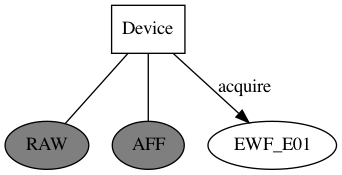
\includegraphics[width=.5\textwidth]{figures/device-to-image.png}
  \caption[Focus on EWF\_E01]{The default image format is EWF\_E01.}
  \label{fig:ewfe01}
\end{figure}

As shown in \cref{fig:ewfe01} the default file format for forensic images in the Lower Saxony Police is the Expert Witness Format (EWF\_E01). \cite{EWF}

Hellonium has to be able to process this file format.

\section{User interface}
\label{sec:gui}

In order to provide access to Hellonium for the less technically experienced investigators, it has to contain some kind of graphical user interface (GUI).

\section{Open Source}
\label{sec:oss}

Open source should be preferred. On the one hand, this allows Hellonium to be assembled according to the modular principle and, on the other hand, all functionalities can be checked using the source code.

\section{Metadata}
\label{sec:metadata}

The user has to be able to identify that the forensic image belongs to the case he is currently working on. To do this, Hellonium has to be able to extract the metadata embedded in shell of the EWF\_E01 container.

\section{Verification}
\label{sec:verification}

\subsection{EWF\_E01}

In order to ensure that the chain of custody is unbroken and the evidence integrity is untouched (digital forensic process), Hellonium must be able to calculate hash values over the contents of the EWF\_E01 container. The result has to be compared with the hash values stored in the metadata from the shell of the EWF\_E01 container. It has be pointed out if they do not match.

Following current, widely used forensic software, at least the hash variants MD5 and SHA1 must be supported.

\subsection{Digital signatures}

To prevent an unauthorised person from manipulating the evidence unnoticed and subsequently creating a new forensic image including new hash values, Hellonium has to be able to verify digital signatures. \cite{Nikkel2016:154}

Signify \cite{Signify}, minisign \cite{Minisign}, GnuPG \cite{GnuPG} and s/mime \cite{SMIME} are widely used. At least one system has to be supported.

\subsection{RFC-3161 Timestamping}

In addition, to prevent also an authorised person from manipulating the evidence unnoticed afterwards and subsequently creating a new forensic image including new hash values, Hellonium has to be able to verify timestamps according to RFC-3161. \cite{Nikkel2016:154}

\section{Direct access storage device}
\label{sec:dasd}

A Direct access storage device (DASD) is one on which each physical record has a discrete location and a unique address. Thus records can be stored on a DASD in such a way that the location of any one record can be determined without extensive searching. Records can be accessed directly as well as serially. \cite{IBM1974}

In the case of the Master's thesis, this basically means hard disk drives and solid state disks.

\subsection{Partition scheme}

A partitioning scheme is a logical structure that are required for the operating system to access the storage space on the physical device. Logical structures include partition tables such as an master boot record (MBR) or GUID partition table (GPT). \cite{Aarnes2017:156}

Both partition schemes have to be interpretable.

\subsection{Partition Table}

During the creation of a partition, an ID (MBR) or a GUID (GPT) is specified, which is intended to save the information which file system will later be used in that partition, but does not necessarily have to.

\begin{figure}[htbp]  % order of priority: h here, t top, b bottom, p page
  \centering
  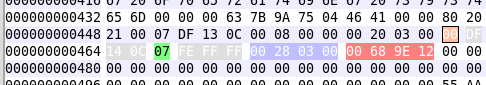
\includegraphics[width=.5\textwidth]{figures/wxhexeditor-mbr-ntfs.png}
  \caption[NTFS partition entry in MBR]{The screenshot shows a partition entry of a NTFS partition in a MBR.}
  \label{fig:NTFSMBR}
\end{figure}

The green marked ID (07) in \cref{fig:NTFSMBR} indicates that the partition is to be formatted with an NTFS file system.

Since the type of partitioning of the DASD, based on the entries in the partition table, can already provide the first clues about operating systems that may be contained, Hellonium has to be able to correctly interpret the structure of data carriers with a Master Boot Record (MBR) as well as a Globally Unique Identifier Partition Table (GPT).

On Apple Macintosh devices with Bootcamp, a hybrid MBR can lead to confusion in this context. \cite{HybridMBR}

This circumstance must also be taken into account in Hellonium.

\subsection{Deleted partitions}

Hellonium has to be able to recognise if partitions have been set as new (empty) or non-existent (deleted) in the partition table in order to hide the relevant areas. Likewise, it has to be able to identify partitions that have only been quick formatted with another file system.

If such system volumes can be successfully restored, it should also be possible to boot from them again.

\section{Read only access}
\label{sec:readonly}

For information retrieval (preview/triage) only forensic tools should be used that require read access to the forensic image.

However, if partitions, file systems, RAID arrays or LVM2 volumes have to be recovered, write access has to be enabled in a forensic sound manner.

At the latest for emulating or virtualising an operating system contained in a forensic image, write access is required in the same way.

\section{Volumes}
\label{sec:volumes}

\subsection{File systems}

A file system stores data on a device so data can be retrieved by the system or a user. File systems are largely independent of an operating system (OS), and different file systems can be supported on different OSs when necessary drivers are installed. \cite{Aarnes2017:160}

It has to be possible to interpret as many file systems as possible.

\begin{figure}[htbp]  % order of priority: h here, t top, b bottom, p page
  \centering
  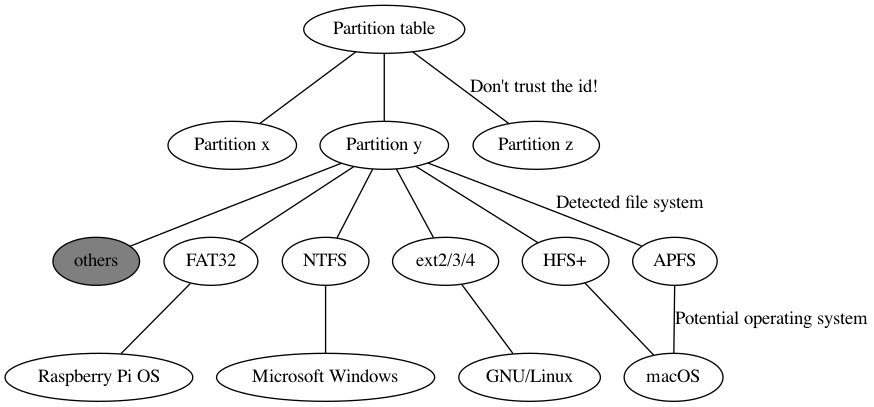
\includegraphics[width=.5\textwidth]{figures/fs-vs-os.png}
  \caption[File system and operating system]{The file system is one hint for the operating system.}
  \label{fig:fsandos}
\end{figure}

In addition to the partition table, it has to be possible to identify a file system in the partition itself, since both specifications do not necessarily have to match. An incorrect specification of the file system in the partition table can prevent Microsoft Windows from starting. GNU/Linux, BSD and Unix are not affected by this restriction. On the basis of the actual file system, one can narrow down or even determine the containing operating system analogous to the partition table. The tool used must therefore be able to recognise not only mainstream, i.e. FAT32 and NTFS, but also HFS+, APFS and ext2/3/4. Support for even more file systems is welcome.

\subsection{Root directory}

The folders contained in the root-directory can strengthen or weaken initial assumptions about the contained operating system.

\subsection{Certain files}

The simple presence of certain files can also strengthen or weaken initial assumptions about the operating system they contain. In addition to a direct interpretation of the contents, it must also be possible to extract them for further external processing.
In order to ensure the chain of custody and evidence integrity (digital forensic process) even after extraction, it must be possible to easily create hash values for the extracted data.
The content of certain files can even substantiate the assumptions regarding the version/release.
For this purpose, the tool used must not only be able to interpret the Windows Registry (mainstream). It must also be able to interpret plist (macOS) and simple text files (GNU/Linux).

\section{Files}
\label{sec:files}

For later successful virtualisation, not only the version of the operating system is interesting. An older version may require a different recipe than a current version. 
However, not everything is needed that is often used for preview or triage. 

\section{Password}
\label{sec:password}

Every secured computer system must require all users to be authenticated at login time. After all, if the operating system cannot be sure who the user is, it cannot know which files and other resources he can access. Password protection is based on something the user knows. The simplest implementation just keeps a central list of logins and passwords. The login typed in is looked up in the list. If they match, the login is allowed. \cite{Tanenbaum2014:626}

In modern operating systems, passwords are not stored in plain text. They are converted to so-called hash values using mathematical one-way functions before they are stored.

Hellonium should offer several ways to find or calculate passwords from hints or against hash values.

\subsection{Microsoft Windows}

In addition to the Windows version, the time zone, password information and network configuration can be read from the Windows registry.
When reading out the password hash values, it must be ensured that both the old (before Windows 10 Anniversary Update) and the new (as of Windows 10 Anniversary Update) procedure for storing the hash values in a hidden manner is supported.

\subsection{Apple macOS}

The information about the operating system version, the time zone, the password instructions and the password hashes are stored under macOS in so-called plists (plain text or binary XML files). Hellonium has to be able to interpret both versions.

At least the last three forms (up to 10.6, 10.7 and from 10.8) of password hashes hast to be correctly extracted from the plists.

If autologin is enabled, the password of the user who is automatically logged in is obfuscated and stored in the file /private/etc/kcpassword. Hellonium has to be able to defuscate the password.

\subsection{GNU/Linux}

Under GNU/Linux it often happens that after successful virtualisation you find yourself on the command line and not on a graphical desktop.
In this case it is good to know which operating system you are dealing with and which steps have to be taken so that the graphic desktop can be reactivated afterwards.

The information about the operating system version and the password hashes can be directly taken from plain text files.

The information about the time zone has to be obtained via the copy or a symbolic link to a corresponding zone file in /usr/share/zoneinfo. Hellonium has to be able to correctly determine the time zone.

\subsection{Raspberry Pi}

In addition, in the case of a Raspberry Pi, it is important to be able to find out the CPU and kernel version, as an appropriately prepared kernel has to be "injected" from the outside. 

If the kernel is incompatible with the original kernel, it may not be possible to load kernel modules afterwards.

Hellonium should already hold a selected choice of kernel versions for this purpose.

\section{Write access}
\label{sec:writeaccess}

Write access in a forensically sound manner is required as soon as changes to a corrupted partition table or file system are necessary.

Likewise, if login passwords need to be cleared.

In the case of an older version of Windows (XP, Vista or 7), the registry have to be changed in order to prevent the Blue Screen of Death (BSOD) immediately after start-up.

Under macOS, a new account with administrator rights can be created by just deleting the file /private/var/db/.AppleSetupDone.

\section{Virtualization}
\label{sec:virtualization}

Depending on the operating system and/or operating system version, the correct choice of virtual hardware also influences whether the system can be booted successfully or not.

It must at least be possible to boot Microsoft Windows, Apple MacOS and GNU/Linux incl. Rapberry Pi OS.

\subsection{Firmware}

\begin{figure}[htbp]  % order of priority: h here, t top, b bottom, p page
  \centering
  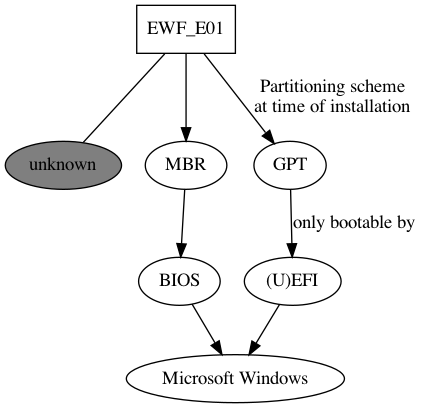
\includegraphics[width=.5\textwidth]{figures/ps-vs-firmware-win.png}
  \caption[Windows fireware dependency]{Micosoft Windows doesn'l like firmware switching.}
  \label{fig:firmware}
\end{figure}

Because Microsoft Windows can only be booted with a BIOS if it was installed with it and can only be booted with a UEFI if it was installed with it, it has to be possible to boot a guest OS with both a BIOS and a UEFI.

\subsection{Network card}

For older operating systems, it should be possible to provide an older network card that is as widely used as possible, as no drivers may have been installed for newer ones.
For newer operating systems, it should be possible to provide a new, current network card that is as widespread as possible, as drivers for older ones may no longer be available for current operating systems.

To prevent unnecessary restarts, the network card should always be available from the beginning.

However, to prevent e.g. remote wiping or the spread of potentially existing malware, the virtual network cable should not be connected by default. A connection should be possible after checking during operation.

\subsection{CPU}

In particular, older 32-bit versions of Windows, which were installed on hardware with only one processor core, occasionally fail to start on a 64-bit system with several cores.

It has to be possible to adjust the CPU in relation to 32- or 64-bit, cores and threads.

\subsection{Apple SMC}

Without this chip, virtualisation of Apple macOS is not possible.

So it has to be possible to offer the chip virtually with correct data.

\subsection{ARM}

A full virtualisation of ARM is unfortunately not possible on Intel/AMD because they are not binary compatible.

Since the Raspberry Pi with ARM SoC has become very popular and is increasingly used as a home server, it has to be possible to emulate an ARM SoC.

\subsection{NVMe}

In some GNU/Linux installations it happens that in /etc/fstab disks are still addressed with device names and not with a label or a UUID. If NVMe is used the name of the device differs from the other ones.

To enable virtualisation without additional changes in the file system, at least IDE, SATA, SCSI, SAS and NVMe controllers should be offered.

\section{Drivers}
\label{sec:drivers}

To enable a display without unnecessary delays and to be able to adjust the resolution beyond VGA resolution, appropriate drivers should be offered for the virtual graphics cards if possible.

\section{Export}
\label{sec:export}

In principle, Hellonium should be user-friendly that remote access or export of the virtual machine should no longer be necessary.

It can still be offered.

\chapter{Technical design}
\label{chap:techdesign}

\section{Operating system}

Since Microsoft Windows and Apple MacOS are not open source operating systems, they cannot be considered as a basis for Hellonium.

Due to the author's insufficient experience with BSD, it was not considered.

The author has been able to gather extensive experience with GNU/Linux for over 20 years. On the server side he has favoured Debian GNU/Linux for years and on the client side he currently favours Arch Linux.

Due to a major change in the Debian project regarding the creation of live systems for optical media, the process is currently somewhat easier under Arch Linux with the \glqq{}archiso\grqq{} \cite{Archiso} tool.

Until the development is completed, an external SSD can be used with Arch Linux \cite{ArchLinux}.

\section{Software}

Since Debian GNU/Linux is rather conservative in terms of package versions and only releases a new version about every two years, Arch Linux was given preference. It has been shown that up-to-date software is necessary, especially for MacOS guests. Arch Linux follows the rolling release and is thus always very up-to-date.

Basically all necessary tools are available as packages for Arch Linux.

Should this not be the case, own recipes can be made available via the Arch Linux User Repository (AUR) \cite{AUR}.

Only in exceptional cases should internal software solutions be used. However, these must not be published via AUR as a matter of principle.

\section{GUI}

User-friendliness already begins with the graphical desktop. This should be preconfigured as well as possible for the intended use.

Since an independent development of a GUI would have exceeded the time frame of the thesis, the possibility was chosen to supplement the file manager Nautilus from the Gnome project with scripts. In order not to have to fulfil any unnecessary dependencies and to ensure the most error-free integration of the file manager possible, the choice of the desktop interface fell on Gnome. The development took place under version 3. However, initial tests have not revealed any problems with version 4 \cite{Gnome}.

\begin{figure}[htbp]  % order of priority: h here, t top, b bottom, p page
  \centering
  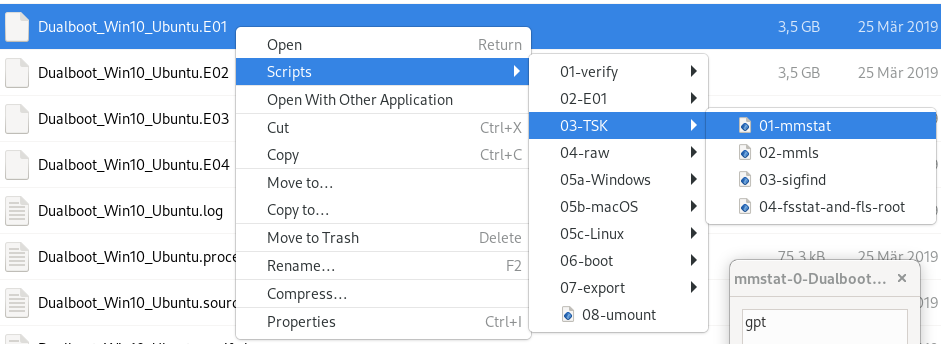
\includegraphics[width=.5\textwidth]{figures/mmstat-gpt.png}
  \caption[Nautilus script example]{The screenshot shows a nautilus script to get the partition scheme.}
  \label{fig:NautilusScript}
\end{figure}

As can be seen in \cref{fig:NautilusScript} , after right-clicking on an EWF\_E01 image, one can select the later functionalities of Hellonium under Scripts.

In the implementation phase, the goal is to find or package the right tools and make them easy to use via Nautilus script.

As can be seen in \cref{fig:xmount}, the user can be asked for further details from a Nautilus script via Zenity \cite{Zenity}.

Unfortunately, this workaround requires the user to interpret the output of each Nautilus script and then decide which script to run next.

\section{Scripts}

Nautilus scripts are like simple shell scripts, which is why shell scripting makes up most of the development. Shell scripting was an important part of the IMT4012-PHS module hosted by Prof. Dr. Fergus T. Toolan.

If no suitable tool exist for individual requirements, it also has to be developed.

The author has already developed Python scripts for digital forensics under Prof. Dr. Fergus T. Toolan in the IMT4505-PHS module of the study.

Therefore, additional tools are basically developed as shell or Python scripts.

While developing Nautilus or shell scripts, the author has followed Fritz Mehner's Bash Style Guide and Coding Standard as closely as possible. \cite{Mehner2014}

\section{Persistence}

All results generated by the Nautilus scripts are stored 1:1 as simple text files in a temporary directory.

The Nautilus scripts check whether they can display an existing file or whether they have to create it first. A result file containing errors can simply be deleted to create a new one.

This is the simplest type of persistence.

\chapter{Development process}
\label{chap:devproc}

\section{Theory}

Prior to his employment, the author worked for several years in software development at the Central Police Department of the Lower Saxony Police, including as an administrator, developer, requirements analysis officer and project manager in projects with five to over 80 project members.

As a rule, the waterfall model with several interactions was used.

In the case of particularly important completed projects, further development was continued in follow-up projects.

Since different projects had to be worked on at the same time, individual employees or entire teams were regularly involved in several projects.

The office was structured in a matrix organisation, in which there were separate teams for requirements management, requirements analysis, server-side development, client-side development, final development of graphical interfaces, database modelling, test laboratory, implementation management including the creation of manuals, public relations, etc.

Communication and discipline were another important cornerstone for successful projects.

\section{Practice}

For the preparation of a practical master thesis as a single person in their spare time, access to a comparable structure was not possible.

One person has to carry out all tasks alone. Communication with other project members is not possible or does not exist. It is also not possible to work uninterruptedly on the project for weeks at a time, as work and family have to be attended to in parallel.

It has proven practical to break down the big picture into smaller parts, as is done in Extreme Programming, in order to be able to use the free time as effectively as possible.

\section{Versioning}

A Gitea repository is used for the development: \url{https://git.neumannsland.de/casualscripter/Masterthesis}
\chapter{Implementation}
\label{chap:implementation}

For the sake of better understanding, only the parts from a Nautilus script that are essential for solving the problem have been included in a listing. The complete script can be found in the Gitea repository.

For better readability, the listings have been individualised by replacing the variables with concrete values.

The short explanations of the command line programs were mostly taken from their manual pages.

If there is no manpage, the description was taken from a readme file (or similar) in the sources.

The reference to the source code was included to prove that it is indeed open source software.

\section{Function library}

It became apparent very early on that it makes sense, in order not to repeat oneself (DRY), to outsource repeatedly used script parts to shell functions. Even better into a separate file: the function library.

The function library contains the following features and functions:

\subsection{trim}

During the development it turned out that some tools output unwanted spaces at the beginning or at the end.

For this reason, the trim function was created.

It removes leading and trailing whitespace characters from a string.

\subsection{Binaries}

Assignments of binary locations automatically/manually to readonly vars for more flexibility or more security.

An example is given in \cref{lst:bin-assign}.

\begin{lstlisting}[
    caption={Examples of the assignment of binaries to variables},
    label=lst:bin-assign,
    language=bash]
readonly WHICH_BIN="/usr/bin/which"
[...]
readonly AWK_BIN="$( ${WHICH_BIN} awk )"
[...]
readonly SIGFIND_BIN="/usr/local/bin/sigfind"
[...]
\end{lstlisting}

\subsection{Parameter}

Unfortunately, the varialbe in Nautilus scripts that contains the transferred file contains a line break at the end.

To avoid problems afterwards, the line break should always be removed.

The functon library removes the newline from NAUTILUS\_SCRIPT\_SELECTED\_FILE\_PATHS (see \cref{lst:guiorcli}).

\subsection{Variable}

If a raw image mounted via xmount has been selected, it is located in a virtual directory in which it is not possible to write.

In this case, the working directory must be changed to a directory with write permissions.

In such a case the functon library sets the variable DIRNAME to a writable location.

\subsection{Messageboxes}

In principle, all output from programs on the command line is hidden behind the Nautilus GUI.

In specific cases, however, the user needs some feedback.

For this case, the functions error\_exit, hint and success have been implemented.

They display messages to the user in zenity message boxes.

\subsection{check\_osr}

The Nautilus scripts were developed under Arch Linux and partly tested on Debian GNU/Linux.

To prevent errors when running on other distributions, the distribution and the release are queried.

If it does not match Arch Linux or Debian GNU/Linux, it will be aborted with a message.

\subsection{check\_dep}

Since it only makes sense to execute a Nautilus script if the tools it calls are available, this is tested at the beginning of each script.

If this is not the case, the script terminates with a corresponding message.

\subsection{check\_xmount\_version}

From xmount 0.5.x to 0.7.x the command line syntax has changed.

If an older version than 0.7.x is installed on the system, the script terminates with a corresponding message.

\subsection{check\_ext}

Because the scripts were developed for different types of images, this function can be used to check the parameter for a corresponding type.

If the type is not correct, e.g. .dd instead of E01, the script terminates with a corresponding note.

\subsection{check\_file}

Some scripts require a file as input and others a directory.

This function can be used to check for an existing file.

If this is not the case, the script terminates with a corresponding message.

\subsection{check\_dir}

This function can be used to check for an existing directory.

If this is not the case, the script terminates with a corresponding message.

\subsection{check\_tmp}

In order for the Nautilus scripts to cache or save their results, the temporary directory has to  exist.

This function checks whether the ./tmp directory exists, creates it if it does no and provides it as variable to the Nautilus script.

\subsection{source\_is\_mounted}

This function is a helper function for other functions.

It checks whether the source passed as parameter is mounted and returns true or false.

\subsection{check\_if\_source\_is\_not\_mounted}

Checks if a device (or image) is NOT mounted and tells the user what to do if it is mounted.

\subsection{check\_if\_source\_is\_mounted}

Checks if a device (or image) is mounted and tells the user what to do if it is not mounted.

\subsection{pwd\_used\_as\_mountpoint}

This function is a helper function for other functions.

It checks whether the current working directory is used as a mountpoint and returns true or false.

\subsection{check\_if\_pwd\_is\_not\_used\_as\_mountpoint}

Checks if the current working directory is NOT a used mountpoint and tells the user what to do if it is used as a mountpoint.

\subsection{check\_if\_pwd\_is\_used\_as\_mountpoint}

Checks if the current working directory IS a used mountpoint and tells the user what to do if it is not used as a mountpoint.

\subsection{check\_if\_is\_looped}

This function checks whether a directory tree has been mounted via loop from a raw image mounted via xmount to prevent accidental changes.

If this is not the case, the script terminates with a corresponding message.

\subsection{disable\_gnome\_automount: }

Hellonium is preset so that new data media are not automatically mounted.

If the Nautilus scripts are also used on another distritbution with Gnome, the automount functionality is prevented as much as possible for forensic reasons.

\subsection{disable\_tracker\_miner}

If a new directory tree is mounted under Gnome, the desktop search automatically starts indexing.

In the case of a complete operating system, this consumes resources unnecessarily. In the worst case, unmounting is blocked for a longer period of time.

For this purpose, this function deactivates the indexing of the Gnome desktop search.

\subsection{xmount\_out\_format}

Asks the user for the output format for xmount (see \cref{fig:xmount}).

\subsection{choose\_partiton}

Asks the user to specify a partition of an image, eg. for mounting.

\subsection{display\_resultfile}

Displays the resultfile of a Nautilus script within a zenity text box.

\subsection{Running checks}

At the end of the library it checks the operating system release and reacts on it, checks that the one and only parameter is only one file and that it is an absolute path to an existing file.

\subsection{Loading}

At the beginning of each Nautilus script, as a second step, it checks whether the function library exists and then loads it (see \cref{lst:source-library}).

\begin{lstlisting}[
    caption={example of checking and sourcing the function library},
    label=lst:source-library,
    language=bash]
readonly LIBRARY="${0%/*/*}/.casualscripter_nautilus-scripts_functions.sh"
if [ ! -f "${LIBRARY}" ] ; then
  zenity --error \
         --text \
         "ERROR: casualscripter_nautilus-scripts_functions.sh MISSING!"
  exit 1
fi

source "${LIBRARY}"
\end{lstlisting}

\section{Verification}

\subsection{EWF\_E01}

libewf \cite{Libewf} by Joachim Metz is a library to access the Expert Witness Compression Format (EWF).

libewf has established itself in the open source environment as a quasi-standard for working with EWF\_E01 files under GNU/Linux.\newline
\newline
\noindent \textbf{ewfverify} is a utility to verify media data stored in EWF files. ewfverify is part ot the project.

\begin{lstlisting}[
    caption={ewfverify example},
    label=lst:ewfverify,
    language=bash]
$ ewfverify -d sha1 -l ./tmp/image.E01.txt ./image.E01
\end{lstlisting}

\noindent The script first checks if the source is an EWF\_E01 image and if the directory tmp is present.

After that it executes ewfverify, writes the output into the log file and waits until it has finished.

The last thing is showing the content of the log file in a zenity window.

\begin{figure}[htbp]  % order of priority: h here, t top, b bottom, p page
  \centering
  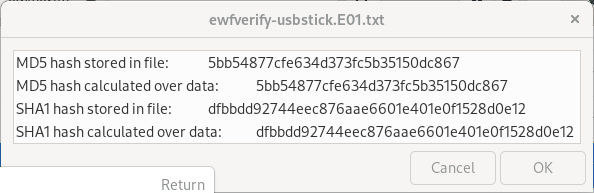
\includegraphics[width=.5\textwidth]{figures/ewfverify.png}
  \caption[ewfverify logfile]{The screenshot shows the content of the logfile of ewfverify}
  \label{fig:ewfverifylog}
\end{figure}

In \cref{fig:ewfverifylog} you can see the open zenity window after successful verification.

If the hash values from the metadata are identical to those calculated over the content, the investigator may continue to use the image.

\subsection{Digital signatures}

\textbf{signify} by Ted Unangst is a small tool for signing OpenBSD OS releases.

It is an open source project \cite{SignifyCSV} hosted by OpenBSD.

The signify utility creates and verifies cryptographic signatures. Not only OS releases.

\begin{lstlisting}[
    caption={signify verify example},
    label=lst:signify,
    language=bash]
$ signify -V -p ./signify-key.pub -m ./image.E01.log
\end{lstlisting}

\noindent If the investigator can read \glqq{}Signature Verified\grqq{}, he can be sure that the person with the publicly available key really created the image.\newline
\newline
\noindent \textbf{minisign} by Frank Denis is a dead simple tool to sign files and verify signatures.

minisign is an open source project hosted at GitHub \cite{Minisign}.

\begin{lstlisting}[
    caption={minisign verify example},
    label=lst:minisign,
    language=bash]
$ minisign -V -p ./minisign.pub -m ./image.E01.log
\end{lstlisting}

\noindent If the investigator can read \glqq{}Signature and comment signature verified\grqq{}, he can be sure that the person with the publicly available key really created the image.\newline
\newline
\noindent \textbf{GNU Privacy Guard} (GnuPG) is a complete and free and open source implementation of the OpenPGP standard.

Among other things, GnuPG allows you to sign your data.

GnuPG can verify data using both embedded (.asc) and separate signature files (.sig). Both variants have been implemented.

The source code of GnuPG is hosted at gnupg.org \cite{GpgGit}.

\begin{lstlisting}[
    caption={gpg separate signature file verify example},
    label=lst:gpg,
    language=bash]
$ gpg --verify ./image.E01.log.sig
\end{lstlisting}

\noindent If the investigator can read \glqq{}Good signature from...\grqq{}, he can be sure that the person with the publicly available key really created the image.\newline
\newline
\noindent \textbf{gpgsm} is part of the GnuPG project.

gpgsm is a tool similar to gpg to provide digital encryption and signing services on X.509 certificates and the CMS protocol. It is mainly used as a backend for S/MIME mail processing. gpgsm includes a full featured certificate management and complies with all rules defined for the German Sphinx project.

\begin{lstlisting}[
    caption={gpgsm s/mime verify example},
    label=lst:gpgsm,
    language=bash]
$ gpgsm --verify ./image.E01.log.pem
\end{lstlisting}

\noindent If the investigator can read \glqq{}Good signature from...\grqq{}, he can be sure that the person with the publicly available key really created the image.\newline
\newline
\noindent All scripts first check if the source is a log file and not the image itself and if the directory tmp is present.

After that they gererate a report with the name of the log file, used signature file, used public key file, md5 and sha1 over the content of the log file.

They start signify, minisign, gpg or pgpsm and adds the output to the report.

At last They show the content of the report in a zenity window .

\subsection{RFC-3161 Timestamping}

The ts command of \textbf{openssl} is a basic Time Stamping Authority (TSA) client and server application as specified in RFC 3161 (Time-Stamp Protocol, TSP).

OpenSSL is an open source project. The project maintains a downstream clone of his git repository on GitHub \cite{OpenSSL}.

In Hellonium \textbf{FreeTSA} \cite{FreeTSA} is used.

FreeTSA trusted timestamping Software as a Service (SaaS) provides an free and easy method to apply RFC 3161 trusted timestamps to time-sensitive transactions through independently verified and auditable date and UTC (Coordinated Universal Time) sources.

\begin{lstlisting}[
    caption={FreeTSA example},
    label=lst:freetsa,
    language=bash]
#!/usr/bin/env bash

curl http://freetsa.org/files/cacert.pem > ./freetsa-org-cacert.pem

openssl ts -verify \
           -in ./image.E01.log.tsr \
           -data ./image.E01.log \
           -CAfile ./freetsa-org-cacert.pem
  
exit 0
\end{lstlisting}

The script first checks if the source is a log file and not the image itself and if the directory tmp is present.

After that it executes curl and openssl and writes the output into the log file.

At last it shows the content of the log file in a zenity window .

If the investigator can read \glqq{}Verification: OK\grqq{}, then he can be sure that the image was created at the specified time.

\section{Metadata}

\textbf{ewfinfo} is a utility to show meta data stored in EWF files.

As ewfverify the ewfinfo tool is also part of the libewf project.

\begin{lstlisting}[
    caption={ewfinfo example},
    label=lst:ewfinfo,
    language=bash]
$ ewfinfo ./image.E01
\end{lstlisting}

\noindent The script first  checks if the source is an EWF\_E01 image and if the directory tmp is present.

After that it executes ewfinfo and writes the output into the log file.

At last shows the content of the log file in a zenity window.

Based on the metadata, the investigator can check whether he is using the correct image for the current case.

\section{DASD}
\label{sec:implementation-dasd}

The Sleuth Kit (TSK) by Brian Carrier is an open source forensic toolkit for analyzing disks and file systems. \cite{Carrier2005:15}

It is the unofficial standard for examining data media or images on the command line under GNU/Linux.

The open source project is hosted at GitHub \cite{TSK}.

\subsection{Partition scheme}

\textbf{mmstat} displays only the partition layout of a volume system.

mmstat is part of the TSK project.

\begin{lstlisting}[
    caption={mmstat example},
    label=lst:mmstat,
    language=bash]
$ mmstat -i ewf ./image.E01
\end{lstlisting}

\noindent Except for the tool that is called by the script, it behaves similarly to the script for ewfinfo.

The investigator should note that at the end of the workflow, he virtualises an image with an MBR with a BIOS and an image with a GTP with a UEFI.

\subsection{Partition table}

\textbf{mmls} displays the layout of the partitions in a volume system, which include partition tables and disk labels.

mmls is also part of the TSK project.

\begin{lstlisting}[
    caption={mmls example},
    label=lst:mmls,
    language=bash]
$ mmls -i ewf ./image.E01
\end{lstlisting}

\noindent Except for the tool that is called by the script, it behaves similarly to the script for ewfinfo.

The ID in the partition table gives a first vague indication of the file system contained in the partition.

If it is probably an Apple operating system, you have to search manually for a hybrid MBR for Bootcamp.

To get the content of a hybrid MBR instead of the content of the GPT you just have to add \glqq{}-t dos\grqq{} to the options.

This is the reason why there are two scripts for mmls.

\subsection{Deleted/overwritten partitions}

\textbf{sigfind} searches through a file (e. g. image) and looks for the hex-signature at a given offset. This can be used to search for lost boot sectors, superblocks, and partition tables.

sigfind is also part of TSK but the author uses a by Rune Nordvik patched version that searches for two signatures at the same time with some of authors own signatures.

To avoid confusion with the original, the author calls it sigfind-ng in the following.

\begin{lstlisting}[
    caption={sigfind-ng example},
    label=lst:sigfind-ng,
    language=bash]
$ sigfind-ng -t fat32 ./image.E01
\end{lstlisting}

\noindent Basically, this script behaves like the others.

As can be seen in \cref{fig:sigfind-ng}, it also asks for the signature to be searched for.

\begin{figure}[htbp]  % order of priority: h here, t top, b bottom, p page
  \centering
  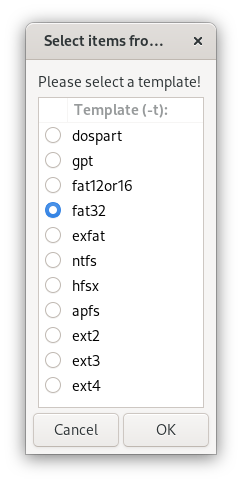
\includegraphics[width=.25\textwidth]{figures/sigfind-ng.png}
  \caption[sigfind(-ng) signatures]{sigfind(-ng) needs a signatur so search for.}
  \label{fig:sigfind-ng}
\end{figure}

If the output indicates that a file system may have been deleted or overwritten, it may be possible to restore it using a writeable raw image.

\subsection{File system and root directory}

\textbf{pstast}, \textbf{fsstat} and \textbf{fls} are also part of TSK.

If the output of mmls suggests that it is an Apple operating system in an APFS, the block of the file system within the APFS container must first be found with pstat.

\begin{lstlisting}[
    caption={pstast example},
    label=lst:pstast,
    language=bash]
$ pstat -i ewf -o 409640 -P apfs image.E01
\end{lstlisting}

With fsstat, the file system presumably contained in the partition should be confirmed.

\begin{lstlisting}[
    caption={fsstat example},
    label=lst:fsstat,
    language=bash]
$ fsstat -i ewf -o 8192 image.E01
\end{lstlisting}

\noindent The last step is then to look with fls into the root directory of the file system.

\begin{lstlisting}[
    caption={fls example},
    label=lst:fls,
    language=bash]
$ fls -i ewf -o 540672 -r -p image.E01
\end{lstlisting}

\noindent Folders such as Windows or \glqq{}Program Files\grqq{} indicate a Windows installation.

Folders such as Applications, Library or System indicate a macOS installation.

Folders such as lib, run or sys indicate a GNU/Linux installation.

If the first partition contains a FAT32 partition with files such as bootcode.bin, kernel.img or start.elf, this indicates a Raspberry Pi OS installation.\newline
\newline
\noindent Basically, this script behaves like the others.

In the main part, it iterates over all partitions and outputs information about the file systems and root directories they contain.

\subsection{Write layer}

\textbf{xmount} by Daniel Gillen allows you to convert on-the-fly between EWF\_E01 and raw format. xmount creates a virtual file system using FUSE (Filesystem in Userspace) that contains a virtual representation of the input image.

In addition, xmount also supports virtual write access to the output files that is redirected to a cache file. This makes it possible to boot acquired harddisk images using QEMU, KVM, VirtualBox, VmWare or alike.
 
The open source project is hosted via the private git repository \cite{xmount} of Daniel Gillen.

\begin{lstlisting}[
    caption={xmount example},
    label=lst:xmount,
    language=bash]
$ mkdir ./mountpoint/
$ xmount --in ewf image.E?? \
         --out raw \
         --cache cache.bin \
         ./mountpoint/
\end{lstlisting}

\noindent As an output format for a virtual hard disk for Qemu/KVM, Hellonium uses the raw format per default.
Since Hellonium is an individualised Arch Linux installation, the user can install Oracle VM VirtualBox \cite{Virtualbox} or VMware Workstation Player \cite{VMware}. In this case, the script also offers the output formats vdi and vmdk (see \cref{fig:xmount}).

\begin{figure}[htbp]  % order of priority: h here, t top, b bottom, p page
  \centering
  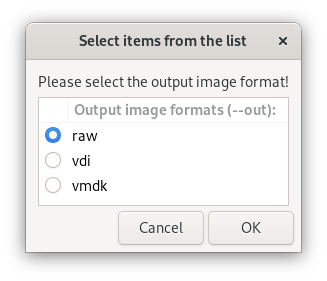
\includegraphics[width=.25\textwidth]{figures/xmount.png}
  \caption[xmount output format]{The Nautilus script asks for the output format.}
  \label{fig:xmount}
\end{figure}

\noindent Basically, this script behaves like the others.

In the main part, it mounts the forensic image using xmount with a write layer as a raw image or virtual hard disk.

Finally, it generates a zenity message window with success or failure.

\subsection{Recover partitions}

\textbf{testdisk} by Christophe Grenier checks and recovers lost partitions.

The open source project is hosted via the private git repository \cite{Testdisk} of Christophe Grenier.

\begin{lstlisting}[
    caption={testdisk example},
    label=lst:testdisk,
    language=bash]
$ testdisk /log /debug ./mountpoint/image.dd
\end{lstlisting}

\noindent First, this script checks whether the specified file is a raw image provided by xmount.

The script starts testdisk in a terminal. This allows the user to operate it as usual.

At last shows the content of the log file in a zenity window.

\subsection{Mount a partition}

The \textbf{mount} command serves to attach the file system found on some device to the big file tree.

The mount command is part of the util-linux package and the source could is hosted at kernel.org \cite{UtilLinux}.

\begin{lstlisting}[
    caption={mount example},
    label=lst:mount,
    language=bash]
#!/usr/bin/env bash

readonly OFFSET="540672"
readonly SIZELIMIT="" # ",sizelimit=..." needed for HFS+
readonly EXTRAS="" # ",revover" for NTFS and ",force" for HFS+

mkdir ./part1/

mount --options loop,rw,offset=${OFFSET}${SIZELIMIT}${EXTRAS} \
      ./mountpoint/image.dd \
      ./part1/

exit 0
\end{lstlisting}

\noindent First, this script also checks whether the specified file is a raw image provided by xmount.

The script asks the user for the partition to be mounted. Then the script mounts this partition per loop.

Finally, it generates a zenity message window with success or failure.

\subsection{Calculate hashes}

To read the data, \textbf{dc3dd} is used.

dc3dd is a forensic patch to the GNU dd program.
dd copies a file and convert and/or formats it according to the operands.

The source code is hostet at SourceForge \cite{Dc3dd}.\newline
\newline
\noindent \textbf{tee} is used to pass the same stream of data to two instances of openssl to compute md5, as well as sha1.

tee is part of the GNU coreutils.

A mirror of the git repository is available over GitHub \cite{CoreUtils}.

\begin{lstlisting}[
    caption={multi hash example},
    label=lst:hash,
    language=bash]
$ dc3dd if=./file.bin \
      | tee >( openssl dgst -md5 -r >> ./tmp/hashes.txt ) \
      >( openssl dgst -sha1 -r >> ./tmp/sha1.tmp' )
$ cat ./tmp/sha1.tmp >> ./tmp/hashes.txt
$ rm ./tmp/sha1.tmp
$ sed --in-place \
      "s/*stdin/*$( basename ./file.bin )/" \
      ./tmp/hashes.txt
\end{lstlisting}

\noindent This script accepts all kind of files as input.

In the main part, it reads the file with dd and creates two hash values at the same time.

At last shows the content of the file with the hashes in a zenity window.

\section{Microsoft Windows}

\begin{figure}[htbp]  % order of priority: h here, t top, b bottom, p page
  \centering
  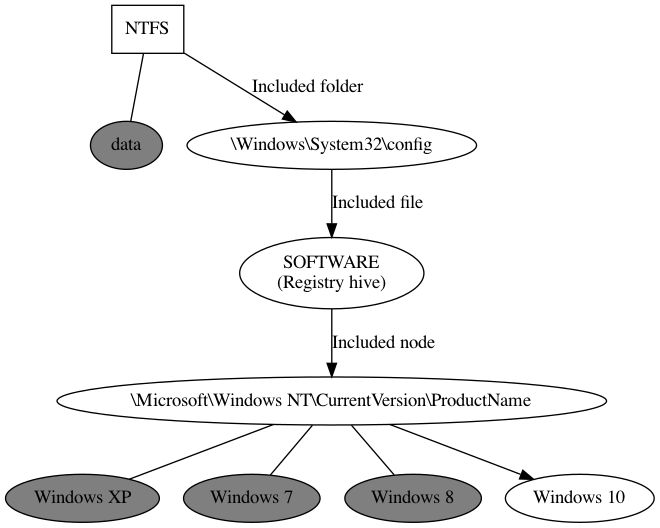
\includegraphics[width=.5\textwidth]{figures/NTFS-to-Win10.png}
  \caption[NTFS and Microsoft Windows]{A Microsoft Windows installation lives in a NTFS.}
  \label{fig:ntfs-win}
\end{figure}

\subsection{Find windows installation and version}

The Windows Registry is a very important artefact. Dealing with this and many other artefacts under Windows was part of the IMT4013-PHS module with Rune Nordvik.\newline
\newline
\noindent \textbf{fcat} opens the named image(s) and copies the file at the path path\_of\_file to standard output.

fcat is also part of TSK.\newline
\newline
\noindent \textbf{hivexget} by Red Hat Inc. is part of the libguestfs project and navigates through a Windows Registry binary "hive" file and extracts either all the (key, value) data pairs stored in that subkey or just the single named data item.

The source code of the project is hosted at GitHub \cite{Libguestfs}.

\begin{lstlisting}[
    caption={hivexget example},
    label=lst:hivexget,
    language=bash]
$ fcat -o 1159168 \
       "/Windows/System32/config/SOFTWARE" \
       ./windows.E01
       > ./tmp/SOFTWARE.hive
$ hivexget ./tmp/SOFTWARE.hive \
           'Microsoft\Windows NT\CurrentVersion' \
           'ProductName' > ./tmp/winver.txt
$ hivexget ./tmp/SOFTWARE.hive \
           'Microsoft\Windows NT\CurrentVersion' \
           'BuildLabEx' >> ./tmp/winver.txt
$ hivexget ./tmp/SOFTWARE.hive \
           'Microsoft\Windows NT\CurrentVersion' \
           'CSDVersion' >> ./tmp/winver.txt
\end{lstlisting}

\noindent The script first checks if the source is an image and and if the directory tmp is present.

It then iterates over all partitions and tries to extract the SOFTWARE hive. If successful, it reads out the Windows version.

At last shows the result in a zenity window.

\subsection{FRED}

Forensic Registry EDitor (\textbf{fred}) by Daniel Gillen is a cross-platform Microsoft Windows registry hive editor.

The open source project is hosted via the private git repository \cite{FRED} of Daniel Gillen.

\begin{lstlisting}[
    caption={fred example},
    label=lst:fred,
    language=bash]
$ fred ./tmp/SAM.hive
\end{lstlisting}

\noindent In a Microsoft Windows XP installation, System32 has to be replaced by system32 (with a lower case s).\newline
\newline
\noindent First, a script checks whether a Windows system directory has been passed and asks the user which registry hive should be opened with FRED.

With another script, the user hive (NTUSER.DAT) can be passed directly.

Finally, the script opens FRED with the corresponding registry hive.

\subsection{BSOD}

\textbf{hivexregedit} exports and merges Registry changes from regedit-format files.

As hivexget it is part of the libguestfs project.

\begin{lstlisting}[
    caption={hivexregedit example},
    label=lst:hivexregedit,
    language=bash]
$ hivexregedit --export \
               --prefix 'HKEY_LOCAL_MACHINE\SYSTEM' \
               ./part2/Windows/System32/config/SYSTEM \
               '\ControlSet001\services\lsi_scsi' \
               > ./tmp/SYSTEM.tmp
$ sed --in-place \
      's/\("Start"=dword:0000000\)\(3\)/\10/' \
      ./tmp/SYSTEM.tmp
$ hivexregedit --merge \
               --prefix 'HKEY_LOCAL_MACHINE\SYSTEM' \
               ./part2/Windows/System32/config/SYSTEM \
               ./tmp/SYSTEM.tmp
\end{lstlisting}

\noindent First, the script checks whether a Windows system directory has been passed.

Then the script exports the SYSTEM hive, changes all services for accessing disks from 3 (Manual) to 0 (Boot) \cite{WindowsServiceStartMode} and merges the changes back.

It informs the user via a zenity message box when the script is finished.\newline
\newline
\noindent For Windows XP, it is recommended to start with the Live System \textbf{OpenGates}.

OpenGates is a small tool written in C that will "open" the hardware limitation "gates" of Windows installations.

The source code is available at the homepage of Daniel Gillen \cite{OpenGates} via an encrypted zip archive.

\subsection{Dump NTLM}

\textbf{creddump7} is a python tool to extract various credentials and secrets from Windows registry hives before and after Microsoft Windows 10 Anniversary Update.

creddump was written by Brendan Dolan-Gavitt, Ronnie Flathers has patched it and Demian Kellermann ported it to Python 3.

The source code is hosted at GitHub \cite{Creddump}.

\begin{lstlisting}[
    caption={creddump7 example},
    label=lst:creddump7,
    language=bash]
$ pwdump.py ./tmp/SYSTEM.hive \
            ./tmp/SAM.hive \
            > ./tmp/pwdump.txt
\end{lstlisting}

\noindent First, the script checks whether a forensic image has been specified.

Then it asks the user for the partition from which the NTLM hash values are to be extracted. Then it extracts the SYSTEM and SAM registry hive and reads the NTLM hash values from them with the help of pwdump (creddump7).

After the output file has been cleaned of system accounts, it is displayed in a zenity message box.

\subsection{Crack NTLM}

\textbf{ophcrack} by Objectif Securite cracks Microsoft Windows passwords (LM and NTLM hashes) with rainbow tables.

The source code is hosted at GitLab \cite{Ophcrack}.

\begin{lstlisting}[
    caption={ophcrack example},
    label=lst:ophcrack,
    language=bash]
$ ophcrack -e -g -n 8 -u \
           -d /var/lib/ophcrack \
           -t vista_free:vista_num:vista_proba_free:vista_special \
           -f ./tmp/pwdump.txt \
           -l ./tmp/ophcrack.log \
           -o ./tmp/passwords.txt
\end{lstlisting}

\noindent \textbf{hashcat} by Jens Steube is the world's fastest and most advanced password recovery utility.

The source code is hosted at GitHub \cite{Hashcat}.

A dictionary attack takes less time. That is the advantage. However, not all possible character combinations are taken into account. That is the disadvantage.\newline
\newline
\noindent \textbf{rockyou.txt} \cite{Rockyou} serves as the dictionary.

\begin{lstlisting}[
    caption={hashcat dictionary example},
    label=lst:hashcat-dict,
    language=bash]
$ hashcat --potfile-disable \
          --hash-type 1000 \
          --attack-mode 0 \
          --workload-profile 3 \
          --optimized-kernel-enable \
          --force \
          --outfile ./tmp/passwords.txt \
          ./tmp/pwdump.txt \
          /var/lib/hashcat/rockyou.txt \
          --rules-file /usr/share/doc/hashcat/rules/dive.rule
\end{lstlisting}

\noindent If time is not an issue, brute force can still be an alternative. Above a certain password length, however, a brute force attack no longer makes sense, even with one or more modern graphics cards!

\begin{lstlisting}[
    caption={hashcat brute force example},
    label=lst:hashcat-bf,
    language=bash]
$ hashcat --potfile-disable \
          --hash-type 1000 \
          --attack-mode 3 \
          --increment \
          --workload-profile 3 \
          --optimized-kernel-enable \
          --force \
          --outfile ./tmp/passwords.txt \
          ./tmp/pwdump.txt \
          "?a?a?a?a?a?a"
\end{lstlisting}

\noindent First, the scripts check whether a text file created via pwdump has been specified.

Depending on the script, ophcrack (rainbow tables) or hashcat (brute force or dictionary attack) is then started and waited until a password is found or the tools have nothing more to do.

Finally, the result file is displayed in a zenity message box.

\subsection{Remove password}

\textbf{chntpw} by by Petter Nordahl-Hagen is a small Microsoft Windows password removal utility.

The source code is available as a zip archive on Petter Nordahl-Hagens homepage \cite{Chntpw}.

\begin{lstlisting}[
    caption={chntpw example},
    label=lst:chntpw,
    language=bash]
$ chntpw -i ./Windows/System32/config/SOFTWARE
\end{lstlisting}

\noindent First of all, the script checks whether a Windows system 
directory has been specified.

The script starts chntpw in a terminal. This allows the user to operate it as usual.

\section{ Apple macOS}

\begin{figure}[htbp]  % order of priority: h here, t top, b bottom, p page
  \centering
  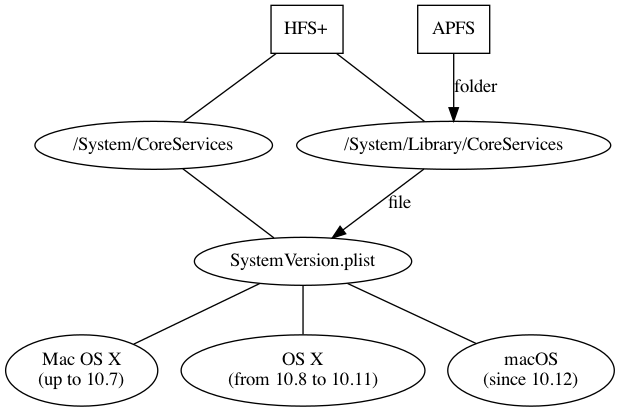
\includegraphics[width=.5\textwidth]{figures/fs-to-macOS.png}
  \caption[APFS/HFS+ and Apple macOS]{An Apple macOS installation lives in an APFS or HFS+.}
  \label{fig:fs-mac}
\end{figure}

\subsection{Plist}

In order to be able to output only certain values for keys from a plist, the author has developed a short Python script.

It is also included in his Gitea repository.

\begin{lstlisting}[
    caption={print\_plist\_entry.py},
    label=lst:ppepy,
    language=python]
def _finditem(obj, key):
  if key in obj: return obj[key]
  for k, v in obj.items():
    if isinstance(v,dict):
      item = _finditem(v, key)
      if item is not None:
        return item

print( key + ":", _finditem( content, key ) )
\end{lstlisting}

\subsection{Find macOS installation and version}

\textbf{ifind}  finds  the meta-data structure that has data\_unit allocated a data unit or has a given file name.\newline
\newline
\noindent \textbf{icat} opens the named image(s) and copies the file with the specified inode number to standard output.

ifind and icat are part of TSK.\newline
\newline
\noindent In an HFS+ file system, you can work directly with an offset. In an APFS file system, the block of the APFS container must be determined beforehand via pstat and then additionally specified with the \glqq{}-B\grqq{} option.

\begin{lstlisting}[
    caption={Get macOS version},
    label=lst:macver,
    language=bash]
$ ifind -o 409640 \
        -B 747286 \
        -n "/System/Library/CoreServices/SystemVersion.plist" \
        ./macOS.E01
$ icat -o 409640 \
       -B 747286 \
       ./macOS.E01 \
       1152921500311972002 \
       > ./tmp/SystemVersion.plist
$ print_plist_entry.py ./tmp/SystemVersion.plist ProductName \
                       > ./tmp/macver.txt
$ print_plist_entry.py ./tmp/SystemVersion.plist ProductVersion \
                       >> ./tmp/macver.txt
$ print_plist_entry.py ./tmp/SystemVersion.plist ProductBuildVersion \
                       >> ./tmp/macver.txt
\end{lstlisting}

\noindent The script first checks if the source is an image and and if the directory tmp is present.

It then iterates over all partitions and tries to extract the SystemVersion.plist. If successful, it reads out the macOS version.

At last shows the result in a zenity window.

\subsection{Timezone}

Depending on the macOS version, there were and/or are different places in the file system where you can find information about the timezone. The simplest is the target pointed to by the symbolic link /private/etc/localtime.

The Nautilus script considers several possibilities.\newline
\newline
\noindent \textbf{istat} displays the uid, gid, mode, size, link number, modified, accessed, changed times, and all the disk units a structure has allocated.

istat is part of TSK.

\begin{lstlisting}[
    caption={get zoneinfo},
    label=lst:zoneinfo,
    language=bash]
$ ifind -o 409640 \
        -B 747037 \
        -n "/private/etc/localtime" macOS.E01
$ istat -o 409640 \
        -B 747037 \
        macOS.E01 \
        4297271160 \
        | grep --extended-regexp "Symbolic.*zoneinfo"
\end{lstlisting}

\noindent The script first checks if the source is an image and and if the directory tmp is present.

It then asks the user for a partition and tries to extract the timezone from /private/etc/localtime (symbolic link), /Library/Preferences.plist for /Library/Preferences/.GlobalPreferences.plist. If successful, it reads out the timezone information.

At last shows the result in a zenity window.

\subsection{Password hints}

User data is located in a different APFS container than the system data.

The password hint can be pulled from the user's plist with print\_plist\_entry.py.

If autologin is activated, the obfuscated password can be defused with \textbf{kcpass.py} by Joaquin Moreno Garijo from /private/etc/kcpassword.

The author has ported the code to python 3.

The source code is hosted at GitHub \cite{Kcpass}.

\begin{lstlisting}[
    caption={defuscate kcpassword},
    label=lst:kcpasswd,
    language=bash]
$ icat -o 409640 
       -B 747037 \
       ./macOS.E01 \
       4297007635 \
       > ./tmp/kcpassword
$ kcpass.py "$( xxd -p ./tmp/kcpassword )"
\end{lstlisting}

\noindent The script first checks if the source is an image and and if the directory tmp is present.

It then asks the user for a partition and tries to extract the plists for real users in the Open Directory and a /private/etc/kcpassword file. After that it extracts the password hints with print\_plist\_entry.py from the user plists and tries to defuscate the kcpassword file with kcpass.py.

At last shows the result in a zenity message box.

\subsection{Dump hash}

The knowledge of how to extract the hash values from different macOS versions is taught by Kurt Helge Hansen in the module IMT4504-PHS.

The learning material is not publicly available.\newline
\newline
\noindent The \textbf{salted SHA1} hash of a macOS installations up to version 10.6 aka Snow Leopard is stored at a specific position of a file.\newline
\newline
\noindent \textbf{cut} prints selected parts of lines from each FILE to standard output.

cut is also part of the GNU coreutils.

\begin{lstlisting}[
    caption={extract hash up to 10.6},
    label=lst:hash106,
    language=bash]
fcat -o 409640 \
     "/private/var/db/shadow/hash/BD3DAA51-38D5-4FED-828E-A51CDB07CF44"  \
     Mac_OS_X.E01 \
     | cut --characters=169-216
\end{lstlisting}

\noindent Dumping the \textbf{salted SHA512} hash of a macOS installation in version 10.7 aka Lion is a bit more difficult.\newline
\newline
\noindent \textbf{plistutil} allows to convert a file in Property List format from binary to XML format or vice-versa.

plistutil is part of the libmobiledevice project.

The source code is hosted at GitHub \cite{Libplist}.\newline
\newline
\noindent \textbf{sed} is a stream editor that is used to perform basic text transformations on an input stream.

sed is part of the GNU project.

the source code is hosted at Savannah \cite{Sed}.\newline
\newline
\noindent \textbf{grep} searches for patterns in each file.

grep is also part of the GNU project.\newline
\newline
\noindent \textbf{tr} translates, squeezes, and/or deletes characters from standard input, writing to standard output.

tr is part of coreutils of the GNU project.\newline
\newline
\noindent \textbf{base64} encode or decode file, or standard input, to standard output.

base64 is part of coreutils of the GNU project.\newline
\newline
\noindent \textbf{xxd} reads a hex dump of a given file or standard input.

xxd is part of the vim project.

vim is hosted at GitHub \cite{Xxd}.

\begin{lstlisting}[
    caption={extract hash 10.7},
    label=lst:hash107,
    language=bash]
$ plistutil --infile ./tmp/user.plist \
  | sed --silent '/ShadowHashData/,/<\/array>/ p' \
  | grep --extended-regexp --invert-match "<.*>" \
  | sed --regexp-extended 's/[[:space:]]//g' \
  | tr --delete '\n' \
  | base64 --decode \
  > ./tmp/shadowhashdata.plist
$ plistutil --infile ./tmp/shadowhashdata.plist \
  | sed --silent '/SALTED-SHA512/,/<\/data>/ p' \
  | grep --extended-regexp --invert-match "<.*>" \
  | sed --regexp-extended 's/[[:space:]]//g' \
  | base64 --decode \
  | xxd -bits -plain \
  | tr --delete '\n'
\end{lstlisting}

\noindent Dumping a Password-Based Key Derivation Function 2 (\textbf{PBKDF2}) derived \textbf{salted SHA512} hash of a macOS installation since version 10.8 aka Mointain Lion is the biggest challenge.\newline
\newline
\noindent \textbf{tail} print the last n lines of each file to standard output.

tail is also part of the GNU coreutils.\newline
\newline
\noindent \textbf{echo} echos the string(s) to standard output.

echo is also part of the GNU coreutils.

The echo at the end of the listing is necessary to prefix the \glqq{}ml\grqq{} to the hash and to separate the individual components from each other using \$ (dollar). Only in this way can hashcat recognise the hash. This is the only way for hashcat to recognise the hash.

\begin{lstlisting}[
    caption={extract hash 10.8 and newer},
    label=lst:hash108,
    language=bash]
$ plistutil --infile ./tmp/tim.plist \
  | sed --silent '/ShadowHashData/,/<\/array>/ p' \
  | grep --extended-regexp --invert-match "<.*>" \
  | sed --regexp-extended 's/[[:space:]]//g' \
  | tr --delete '\n' \
  | base64 --decode \
  > ./tmp/shadowhashdata.plist
$ ITERATION="$( plistutil --infile ./tmp/shadowhashdata.plist \
                | sed -E -n '/SALTED-SHA512-PBKDF2/,/<\/dict>/ p' \
                | grep -F -A1 "iterations" \
                | tail -n 1 \
                | sed -E 's#[[:space:]]*</?integer>##g' )"
$ SALT="$( plistutil --infile ./tmp/shadowhashdata.plist \
           | sed -E -n '/SALTED-SHA512-PBKDF2/,/<\/dict>/ p' \
           | sed -n '/salt/,/<\/data>/ p' \
           | grep -E -v "<.*>" \
           | sed -E 's/[[:space:]]//g' \
           | base64 -d \
           | xxd -b -p \
           | tr -d '\n' )"
$ ENTROPY="$( plistutil --infile ./tmp/shadowhashdata.plist \
              | sed -E -n '/SALTED-SHA512-PBKDF2/,/<\/dict>/ p' \
              | sed -n '/entropy/,/<\/data>/ p' \
              | grep -E -v "<.*>" \
              | sed -E 's/[[:space:]]//g' \
              | tr -d '\n' \
              | base64 -d \
              | xxd -b -p \
              | tr -d '\n' \
              | cut -c 1-128 )"
$ echo "\$ml\$${ITERATION}\$${SALT}\$${ENTROPY}"
\end{lstlisting}

\noindent The scripts first checks if the source is an image and and if the directory tmp is present.

They then ask the user for a partition and try to extract the hashes from a file under /private/var/db/shadow/hash (until 10.6) or from a users plist (since 10.7) with a little bit of comannd line kung fu.

At last they show the result in a zenity message box.

\subsection{Crack hash}

Because the hashes are salted, rainbow tables are not useful.

Given the complexity of the hash values, brute force hardly makes sense for reasons of time and is therefore skipped.

The call of Hashcat is comparable to the one for cracking NTLM (see \cref{lst:hashcat-dict}) hash values. Only the hash types are different. The hash type for salted SHA1 is \textbf{122}, that for salted SHA512 is \textbf{1722} and that for salted SHA512 PBKDF2 is \textbf{7100}.

For the last one, a short dictionary is recommended, as the duration quickly goes into years.

\subsection{Redo setup}

On macOS installations that were installed in an HFS+, the partition can be mounted regularly under GNU/Linux. By deleting the file /private/var/db/.AppleSetupDone, the setup can be gone through again as already directly after the installation. A new user with administrative rights (comparable to root) is created.

On macOS installations that were installed in APFS, this is unfortunately not possible due to the lack of write support for APFS. In this case, the file has to be deleted either in recovery mode or after booting macOS from an external devise.

\section{GNU/Linux}

\begin{figure}[htbp]  % order of priority: h here, t top, b bottom, p page
  \centering
  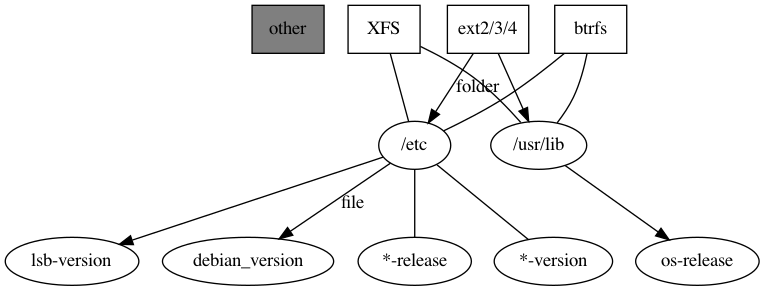
\includegraphics[width=.5\textwidth]{figures/fs-to-Linux.png}
  \caption[File systems and GNU/Linux]{An GNU/Linux installation could live in different file systems.}
  \label{fig:fs-lin}
\end{figure}

\subsection{Find GNU/Linux installation and version}

The versatility of GNU/Linux is both a blessing and a curse. Unfortunately, the name and version of the distribution is not (yet) stored uniformly.

That is why this Nautilus script looks vor
os-release,
debian\_version,
slackware-version,
arch-release,
gentoo-release,
fedora-release,
redhat-release,
SuSE-release,
frugalware-release,
altlinux-release,
mandriva-release,
meego-release,
angstrom-version,
mageia-release and
lsb-release
in /etc.

If several files are found, the user has to interpret the result manually.

\subsection{RPi CPU version}

\textbf{zgrep} invokes grep on compressed or gzipped files.

zgrep is part of the GNU gzip project and hostet at Savannah \cite{Gzip}.\newline
\newline
\noindent \textbf{gawk} is the GNU Project's implementation of the awk pattern scanning and processing language.

gawk is also part of the GNU project and hosted at Savannah \cite{Gawk}.\newline
\newline
\noindent \textbf{sort} writes sorted concatenation of all file(s) to standard output.

sort is also part of the GNU coreutils project.

\begin{lstlisting}[
    caption={identify RPi CPU},
    label=lst:rpicpu,
    language=bash]
$ zgrep --fixed-strings "CPU:" .tmp/kern.log \
  | awk -F "CPU: " '/Processor/ { print $NF; }'
  | sort --unique
\end{lstlisting}

\noindent The script first checks if the source is an image and and if the directory tmp is present.

It then searches the contents of /var/log/kern.log for CPU + Processor in the Linux partition of the Raspberry Pi OS installation.

At last shows the result in a zenity window.

\subsection{RPi kernel version}

\textbf{binwalk} by Craig Heffner is a fast, easy to use tool for analyzing, reverse engineering, and extracting firmware images.

The source code is hosted at GitHub \cite{Binwalk}.\newline
\newline
\noindent \textbf{zcat} uncompresses either a list of files on the command line or its standard input and writes the uncompressed data on standard output.

zcat is also part of the GNU gzip project.\newline
\newline
\noindent \textbf{strings} prints per default the printable character sequences that are at least 4 characters long and are followed by an unprintable character.

strings is part of the GNU binutils project hosted at Sourceware \cite{Binutils}.

\begin{lstlisting}[
    caption={identify RPi kernel version},
    label=lst:rpikernel,
    language=bash]
$ SKIP="$( binwalk ./tmp/kernel.img \
           | awk '/gzip compressed data/ { print $1; }' )"
$ dd if=./tmp/kernel.img bs=1 skip="${SKIP}" status=none \
    | zcat 2>/dev/null \
    | strings \
    | grep -F "Linux version"
\end{lstlisting}

\noindent The script first checks if the source is an image and and if the directory tmp is present.

It then extracts the kernel image from the FAT32 partition of a Raspberry Pi OS, decompresses it and searches for \glqq{}Linux version\grqq{} in the human readable part of the content.

At last shows the result in a zenity message box.

\subsection{Timezone}

GNU/Linux has also adopted different ways of remembering the time zone over time. There are also differences among the distributions.

If you have luck, the time zone is directly in /etc/timezone as plain text.

If not you have to interpret the symbolic link of /etc/localtime or find the origial of the file under /usr/ahre/zoneinfo.

The Nautilus script tries all variants.

\subsection{Dump hash}

Dumping the hashes of a GNU/Linux system is straight forward.

\begin{lstlisting}[
    caption={dump SHA512crypt hashes},
    label=lst:sha512crypt,
    language=bash]
$ awk -F ":" '$2 ~ /.{3,}/ { print $2; }' ./tmp/shadow
\end{lstlisting}

\noindent The script first checks if the source is an image and and if the directory tmp is present.

It then asks the user for a partition and tries to extract the hashes from /etc/shadow.

At last shows the result in a zenity message box.

\subsection{Crack hash}

Because the hashes are salted, rainbow tables are not useful.

Given the complexity of the hash values, brute force hardly makes sense for reasons of time and is therefore skipped.

The call of Hashcat is comparable to the one for cracking NTLM (see \cref{lst:hashcat-dict}) hash values. Only the hash types are different. The hash type for salted SHA512 is \textbf{1800}.

As the latest macOS it needs a year or longer. Only recommended with a short dictionary.

\subsection{Change password}

The \textbf{passwd} command changes passwords for user accounts.

passwd is part of the shadow project.

It is hosted at GitHub \cite{Shadow}.

\begin{lstlisting}[
    caption={Change GNU/Linux password},
    label=lst:passwd,
    language=bash]
$ passwd --root ./part2/ user
\end{lstlisting}

\noindent First, the Nautilus script checks whether a path has been specified. If not, a password would be changed in its own system. This should be avoided.

Then it checks whether the path has been made available by xmount with a write layer and mount with loop to prevent changes to an image.

After that, passwd is called in a terminal window and can be operated as usual.

\section{Virtualization}

QEMU is a generic and open source machine \& userspace emulator and
virtualizer.

The author prefers QEMU to VMware Workstation Player/Pro because it is open source.

Many people are involved in the open source project, which is hosted on  GitLab \cite{Qemu}.

The author prefers QEMU to Oracle VM VirtualBox because it can be completely controlled from the command line. This makes integration into his Nautilus scripts easier. Furthermore, VirtualBox cannot emulate ARM architecture.

\subsection{BIOS}

QEMU uses the PC BIOS from the Seabios project per default.

As you can see in \cref{lst:bios} the option \glqq{}-enable-kvm\grqq{} enables the kernel based virtual machine (KVM) full virtualization support if available.

The VM is configured to pass through the CPU of the host with only one thread and only one core to support older Microsoft Windows XP installations, with 3GB of RAM, with an usb-tablet as a pointer, with QXL paravirtual graphic card including VESA 2.0 VBE support (the drivers can be downloaded from the SPICE project page \cite{Spice}), with a rtl8139 network interface (it is an older, slower but good supported network card on older operating systems) with restricted access to the network and the image as a DASD.

The VM can be controlled with the option \glqq{}-monitor stdio\grqq{}  in the console after startup.

\begin{lstlisting}[
    caption={Quemu BIOS},
    label=lst:bios,
    language=bash]
$ qemu-system-x86_64 \
  -enable-kvm \
  -cpu host \
  -smp 1,cores=1 \
  -m 3072 \
  -usb -device usb-tablet \
  -vga qxl \
  -device rtl8139,romfile="/usr/share/qemu/pxe-rtl8139.rom",netdev=net0 \
  -netdev user,restrict=on,id=net0 \
  -monitor stdio \
  -drive file="./mountpoint/image.dd",index=0,media=disk,format=raw
\end{lstlisting}

\noindent Today it is the easiest way to virtualize a Microsoft Windows installation in Bootcamp.

\begin{figure}[htbp]  % order of priority: h here, t top, b bottom, p page
  \centering
  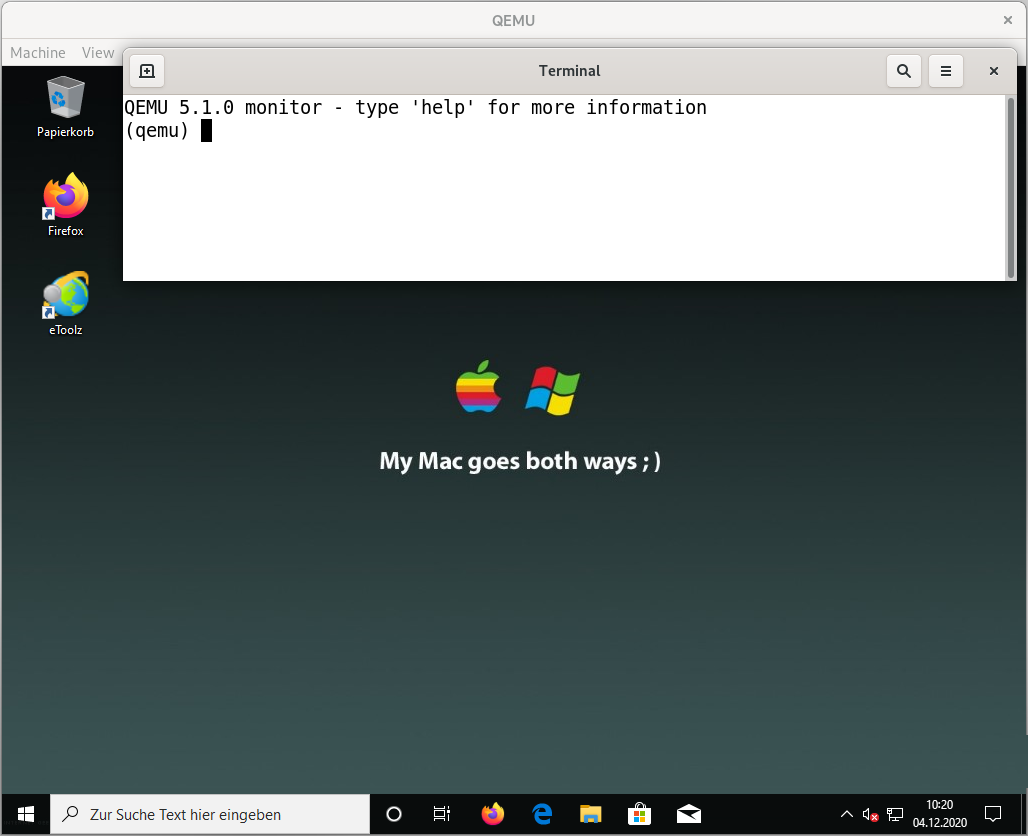
\includegraphics[width=.75\textwidth]{figures/boot-bios-BOOTCAMP.png}
  \caption[Qemu BIOS]{Windows on a Mac (Bootcamp) has to be bootet with a BIOS.}
  \label{fig:bios}
\end{figure}

\noindent First, the Nautilus script checks whether a raw image has been given. This must have been created by xmount with a write layer and no partition should be mounted from it.

Then the image is passed to the call of qemu (see \cref{lst:bios}. If all the previous steps have been done in the right order and interpreted correctly, the result should look like in \cref{fig:bios}.

\subsection{(U)EFI}

OVMF is an EDK II based project to enable UEFI support for Virtual Machines.

The open source project is hosted at GitHub \cite{Ovmf}.

The other options are for fine tuning the powersaving mode and the virtual graphic card.

An example of the command line changes from the previous scripts can be seen in \cref{lst:uefi}.

\begin{lstlisting}[
    caption={Quemu UEFI},
    label=lst:uefi,
    language=bash]
[...]
  -drive file="/usr/[...]/OVMF_CODE.fd",if=pflash,format=raw,readonly \
  -global PIIX4_PM.disable_s3=0 \
  -device qxl-vga,revision=4 \
[...]
\end{lstlisting}

\noindent This configuration is optimal for Microsoft Windows 10 like in \cref{fig:uefi}.

\begin{figure}[htbp]  % order of priority: h here, t top, b bottom, p page
  \centering
  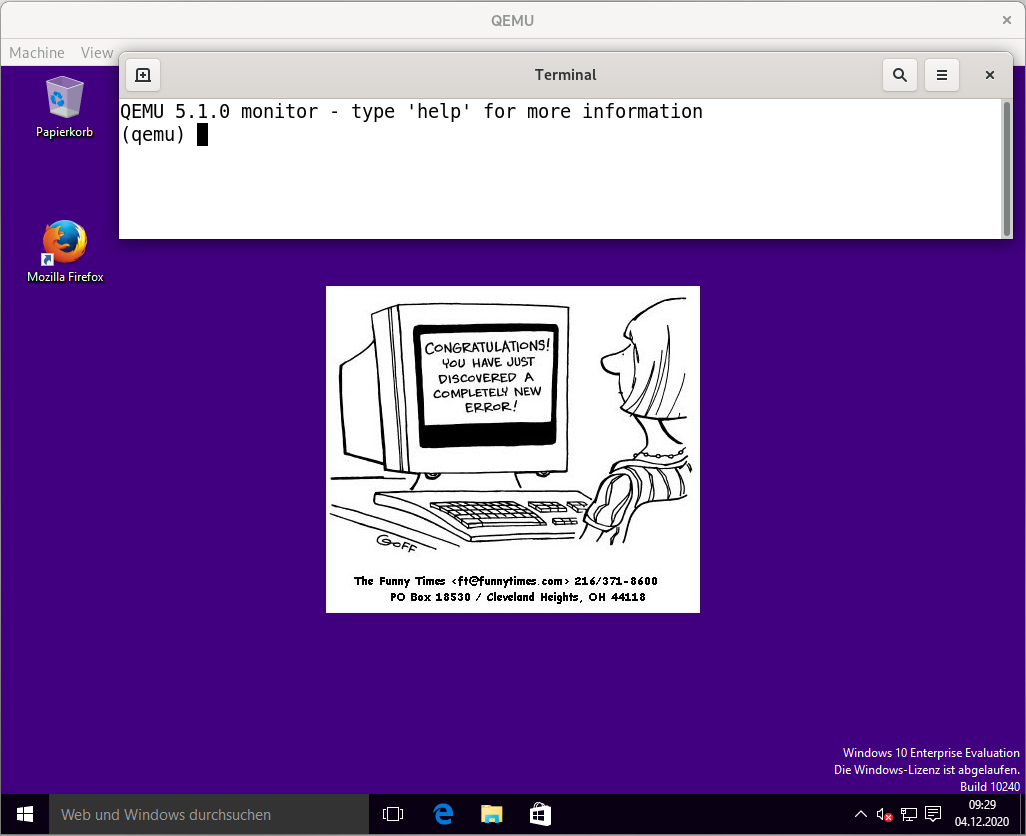
\includegraphics[width=.75\textwidth]{figures/boot-uefi-win10ee-qxl.png}
  \caption[Qemu UEFI]{Windows on a GPT has to be bootet with an UEFI.}
  \label{fig:uefi}
\end{figure}

\subsection{Network}

If the older rtl8139 network card is to old an there are no driveres available anymore, the e1000-82540em will be the better solution on newer systems.

An example of the command line changes from the previous scripts can be seen in \cref{lst:e1000}.

\begin{lstlisting}[
    caption={Quemu new network interface (UEFI)},
    label=lst:e1000,
    language=bash]
[...]
  -device e1000-82540em,romfile="/usr/share/qemu/efi-e1000.rom",netdev=net0 \
[...]
\end{lstlisting}

\subsection{Controller}

The controller is a chip or a set of chips that physically controls the device (e. g. DASD). In many cases, the actual control of the device is complicated and detailed, so it is the job of the controller to present a simpler interface to the operating system. \cite{Tanenbaum2014:28}

If another interface for the drive is needed it can be easily changed.

QEMU is able to provide ide, scsi, sd, mtd, floppy, pflash, virtio or none as an interface.

An example of the command line changes from the previous scripts can be seen in \cref{lst:nvme}.

\begin{lstlisting}[
    caption={Quemu NVMe controller},
    label=lst:nvme,
    language=bash]
[...]
  -drive file=./mountpoint/image.dd,if=none,id=NVME1 \
  -device nvme,drive=NVME1,serial=nvme-1
[...]
\end{lstlisting}

\subsection{Live system}

For starting the system with a live dvd/cd or with a dvd/cd with drivers it is also possible to attach an optical device.

The easiest way to insert a virtual CD/DVD is to use the \glqq{}-cdrom\grqq{} option.

The Nautilus script asks the user for an ISO image.

In the \cref{fig:cdrom} you can see the started Live GNU/Linux system \glqq{}grml\grqq{}.

\begin{figure}[htbp]  % order of priority: h here, t top, b bottom, p page
  \centering
  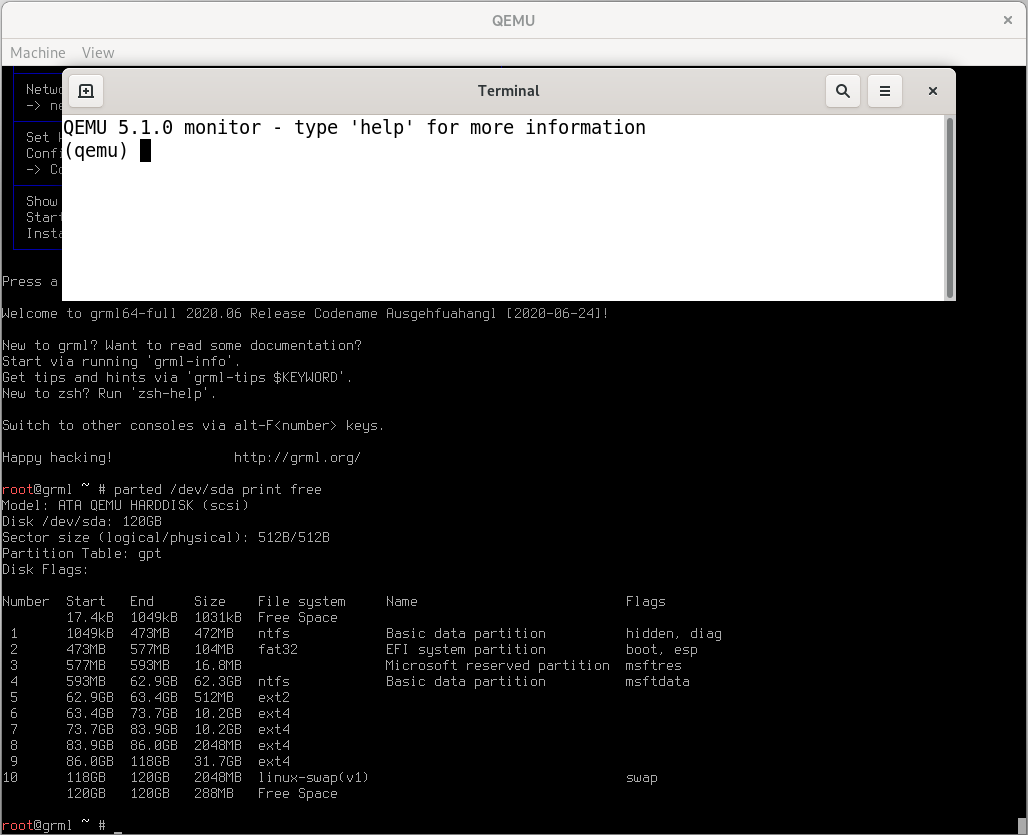
\includegraphics[width=.75\textwidth]{figures/boot-cdrom-grml.png}
  \caption[Qemu with CD/DVD]{Grml bootet with an attached image.}
  \label{fig:cdrom}
\end{figure}

\subsection{Drivers and tools}

A prebuild ISO image with drivers (eg.  QXL drivers) and useful tools (Windows Sysinternals \cite{Sysinternals}, NirSoft \cite{Nirsoft}, BusyBox \cite{Busybox}, Dropbear \cite{Dropbear}, rsync \cite{Rsync}, Find Any File \cite{FindAnyFile}, ...) is included in Hellonium.

There is also a script in Hellonium to update the prebuild ISO if needed.

\begin{lstlisting}[
    caption={Build ISO with drivers and tools},
    label=lst:mkiso,
    language=bash]
$ mkisofs -lJR \
          -o ./drivers-and-tools.iso \
          ./drivers-and-tools/
\end{lstlisting}

\subsection{CPU}

If multiple cpus with multiple threads and multiple cores are needed this is possible too.

An example of the command line changes from the previous scripts can be seen in \cref{lst:smp}.

\begin{lstlisting}[
    caption={Quemu Symmetric multiprocessing},
    label=lst:smp,
    language=bash]
readonly CPU_SOCKETS="1"
readonly CPU_CORES="2"
readonly CPU_THREADS="4"
[...]
  -smp "${CPU_THREADS}",cores="${CPU_CORES}",sockets="${CPU_SOCKETS}"
[...]
\end{lstlisting}

\subsection{macOS up to 10.8}

Especially for the big cats of the macOS operating systems there more fine tuning needed (see \cref{lst:cats}.

The GitHub repository of Dhiru Kholia \cite{OSXKVM}is a good starting point for that.

For more details, please refer to the QEMU manual page and the GitHub repository mentioned above.

\begin{lstlisting}[
    caption={Quemu macOS up to 10.8},
    label=lst:cats,
    language=bash]
$ qemu-system-x86_64 \
  -enable-kvm \
  -cpu core2duo \
  -smp 2,cores=2 \
  -m 3072 \
  -machine q35 \
  -usb -device usb-kbd -device usb-mouse \
  -device isa-applesmc,osk="ourhardwork[...](c)AppleComputerInc" \
  -kernel "Enoch-rev.2922_bootloader" \
  -smbios type=2 \
  -netdev user,id=hub0port0 \
  -device e1000-82545em,netdev=hub0port0,id=mac_vnet0
  -vga std \
  -monitor stdio \
  -device ahci,id=ahci0 \
  -drive id=Macintosh_HD,if=none,format=raw,file="./mountpoint/macOS.dd" \
  device ide-hd,bus=ahci0.0,drive=Macintosh_HD,id=sata-disk0
\end{lstlisting}

\noindent A successful start with login of Snow Leopard can be seen in \cref{fig:cats}.

\begin{figure}[htbp]  % order of priority: h here, t top, b bottom, p page
  \centering
  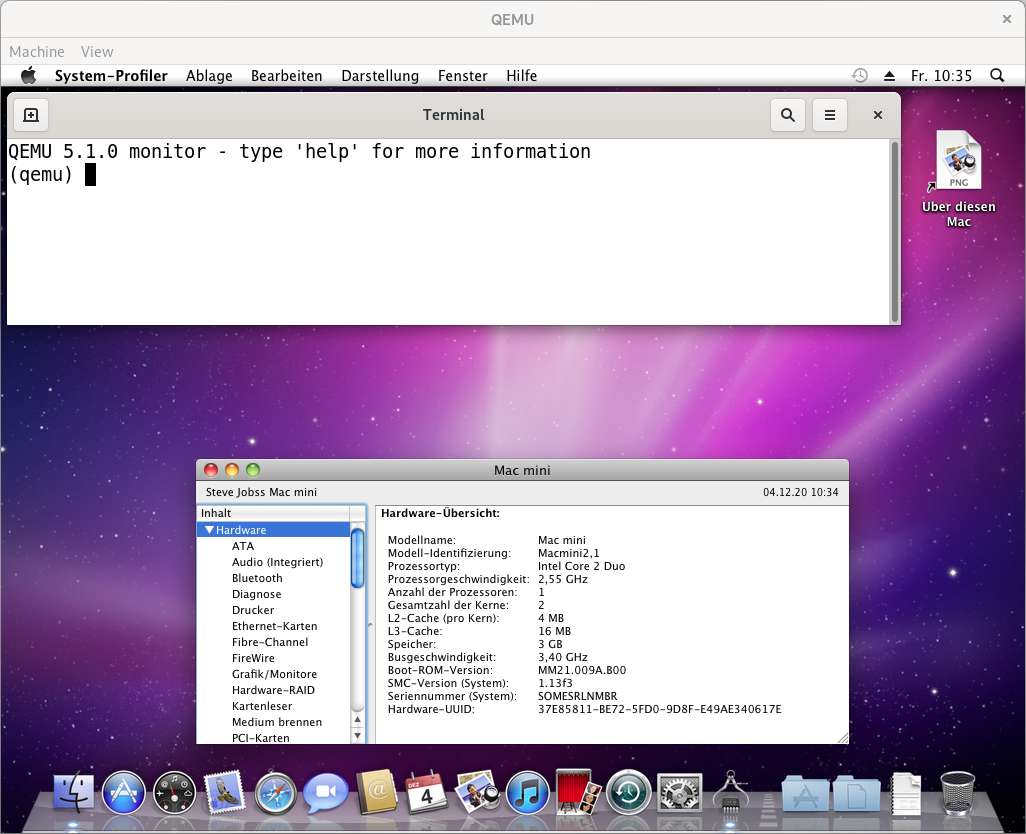
\includegraphics[width=.75\textwidth]{figures/boot-macos-snow-leopard.png}
  \caption[Qemu macOS big cat]{Snow Leopard boots fine with Enoch.}
  \label{fig:cats}
\end{figure}

\subsection{macOS up from 10.9}

With each new macOS version, the configuration becomes more complicated. For the macOS versions with locations in their names, the configuration from \cref{lst:locations} has proven itself so far.

Here, reference is also made to the GitHub repository of Dhiru Kholia.

\begin{lstlisting}[
    caption={Quemu macOS 10.9 and newer},
    label=lst:locations,
    language=bash]
readonly MY_OPTIONS=",+invtsc,vmware-cpuid-freq=on,+pcid,+ssse3,+sse4.2,+popcnt[...]"

$ qemu-system-x86_64 \
  -enable-kvm \
  -cpu Penryn,kvm=on,vendor=GenuineIntel${MY_OPTIONS} \
  -smp 4,cores=2 \
  -m 4096 \
  -machine q35 \
  -usb -device usb-kbd -device usb-mouse \
  -device isa-applesmc,osk="ourhardwork[...]](c)AppleComputerInc" \
  -drive if=pflash,format=raw,readonly,file="${HOME}/Hackintosh/OVMF_CODE.fd" \
  -drive if=pflash,format=raw,file="${HOME}/Hackintosh/OVMF_VARS-1024x768.fd" \
  -smbios type=2 \
  -vga vmware \
  -device ich9-intel-hda -device hda-duplex \
  -device ich9-ahci,id=sata \
  -drive id=Clover,if=none,snapshot=on,format=qcow2,file="./CloverNG.qcow2" \
  -device ide-hd,bus=sata.1,drive=Clover \
  -drive id=MacHDD,if=none,format=raw,file="./mountpoint/macOS.dd" \
  -device ide-hd,bus=sata.2,drive=MacHDD \
  -netdev user,id=hub0port0 \
  -device e1000-82545em,netdev=hub0port0,id=mac_vnet0
  -monitor stdio
\end{lstlisting}

\noindent A successful start with login of Catalina can be seen in \cref{fig:locations}.

\begin{figure}[htbp]  % order of priority: h here, t top, b bottom, p page
  \centering
  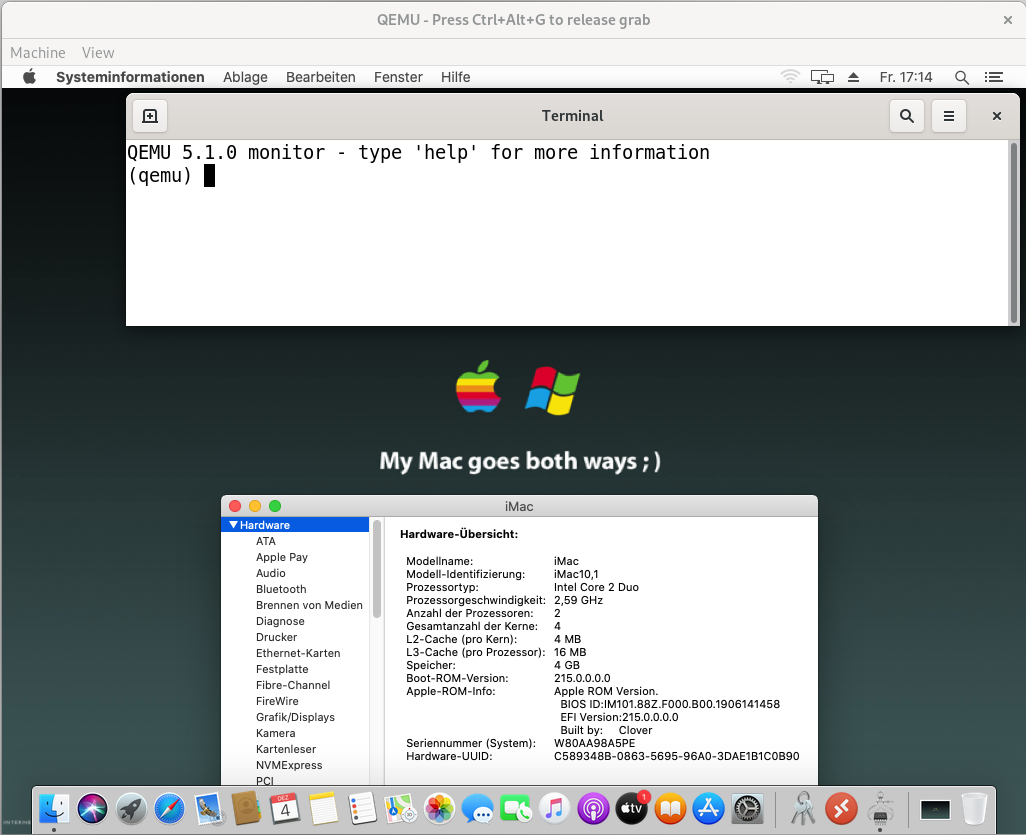
\includegraphics[width=.75\textwidth]{figures/boot-macos-catalina.png}
  \caption[Qemu macOS location]{Newer macOS needs more bleeding edge features.}
  \label{fig:locations}
\end{figure}

\subsection{RPi with cli}

A Raspberry Pi OS can be emulated by specifying the machine \glqq{}virt\grqq{} \cite{QemuARM}.

However, this requires a suitable Linux kernel with virtio support.

For this purpose Hellonium contains a selection of prebuild Linux kernels with virtio support.

If a kernel is missing in the future, the script (see \cref{app:scripts}) only needs to be adapted accordingly.

The complete command line call can be taken from \cref{lst:cli}.

\begin{lstlisting}[
    caption={Quemu RPi CLI},
    label=lst:cli,
    language=bash]
readonly CMDLINE="$( fcat -o 8192 "/cmdline.txt" ./rpi.E01 \
                     | sed 's/tty1/ttyAMA0/' )"
$ qemu-system-arm \
  -kernel "${HOME}/RPi/4.19.97/RPi2-kernel7-virtio" \
  -append "${CMDLINE}" \
  -m 1024 \
  -M virt \
  -cpu cortex-a7 \
  -drive file="./mountpoint/rpi.dd",format=raw,if=none,id=hd-root \
  -device virtio-blk-device,drive=hd-root \
  -netdev user,id=mynet \
  -device virtio-net-device,netdev=mynet \
  -object rng-random,filename=/dev/urandom,id=rng0 \
  -device virtio-rng-pci,rng=rng0 \
  -nographic \
  -no-reboot
\end{lstlisting}

\noindent A successful start of a Raspberry Pi OS with an external virto kernel can be seen in \cref{fig:cli}.

\begin{figure}[htbp]  % order of priority: h here, t top, b bottom, p page
  \centering
  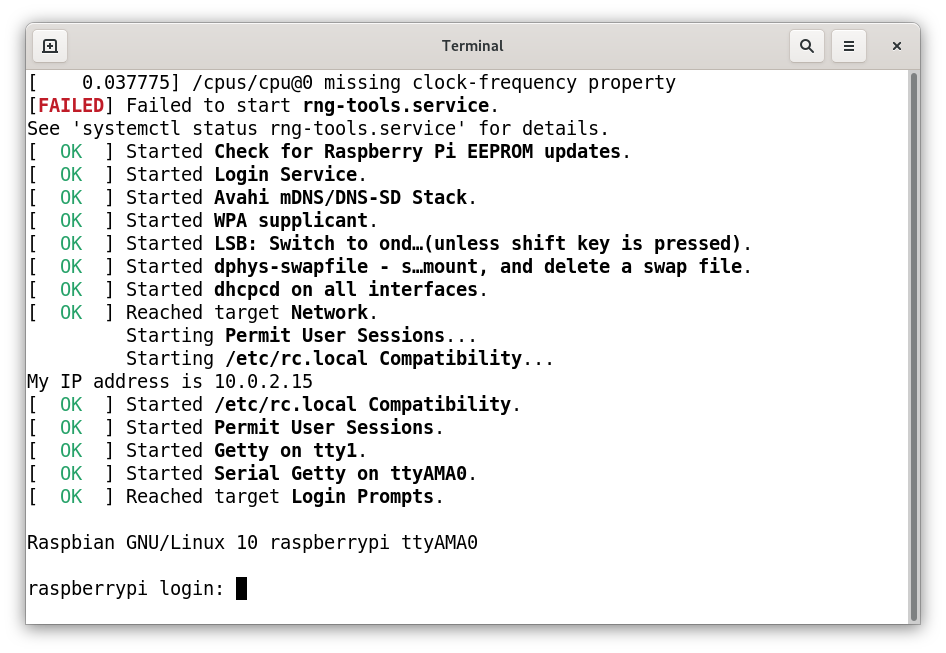
\includegraphics[width=.5\textwidth]{figures/boot-rpi-with-cli-only.png}
  \caption[Qemu RPi CLI]{CLI should be faster with more RAM.}
  \label{fig:cli}
\end{figure}

\subsection{RPi with GUI}

If the original system was used with a graphical interface, another machine has to be used for emulation.

The \glqq{}versatilepb\grqq{} machine was/is quite useful for this.

Unfortunately, the memory is limited to 256MB. Currently, Raspberry Pis with up to 8GB of memory are available. That could become a problem in the future.

However, you also need an appropriate kernel for this. The kernels from Dhruv Vyas' GitHub repository \cite{Versatilepb} basically fulfil this purpose.

The complete command line call can be taken from \cref{lst:gui}.

\begin{lstlisting}[
    caption={Quemu RPi GUI},
    label=lst:gui,
    language=bash]
$ qemu-system-arm \
  -M versatilepb \
  -cpu arm1176 \
  -m 256 \
  -drive file="./mp/rpi.dd",if=none,index=0,media=disk,format=raw,id=disk0 \
  -device virtio-blk-pci,drive=disk0,disable-modern=on,disable-legacy=off \
  -net nic \
  -net user \
  -dtb "${HOME}/RPi/versatilepb/versatile-pb-buster-5.4.51.dtb" \
  -kernel "${HOME}/RPi/versatilepb/kernel-qemu-5.4.51-buster" \
  -append 'root=/dev/vda2 panic=1' \
  -no-reboot
\end{lstlisting}

\noindent A successful start of a Raspberry Pi OS and login with the alternative hardware empulation can be seen in \cref{fig:gui}.

\begin{figure}[htbp]  % order of priority: h here, t top, b bottom, p page
  \centering
  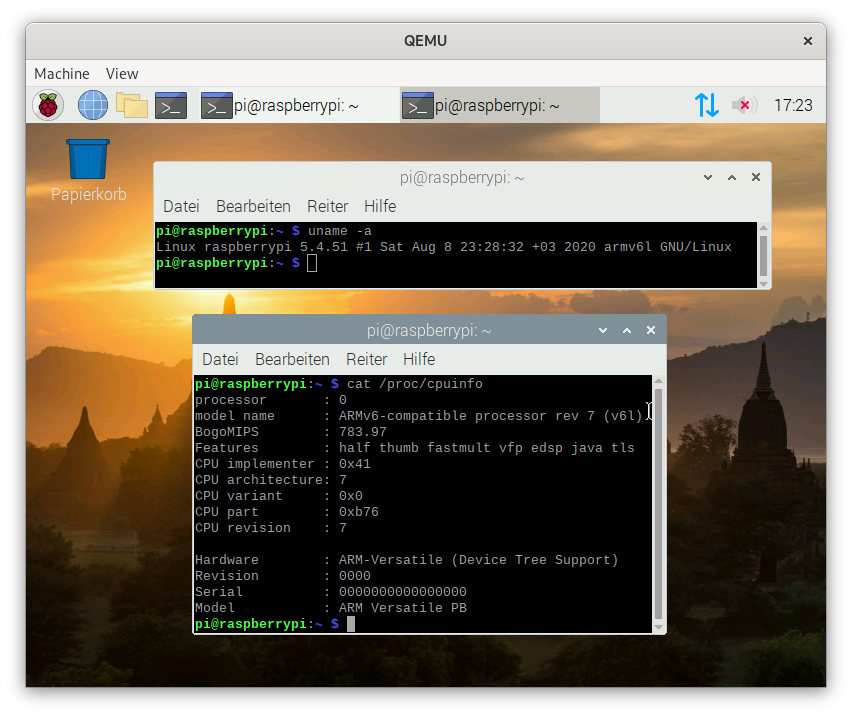
\includegraphics[width=.75\textwidth]{figures/boot-rpi-with-gui.png}
  \caption[Qemu RPi GUI]{GUI mode is slower with less RAM but more beautiful.}
  \label{fig:gui}
\end{figure}

\section{Sharing}

\subsection{VNC}

Virtual Network Computing (\textbf{VNC}) shares the tty or the desktop of a virtual machine over the network.

A VNC server is included in QEMU.

The Nautilus scripts for virtualize or emulate an image are asking if the user want to enable VNC.

\subsection{Export}

\textbf{qemu-img} allows you to create, convert and modify images offline.

qemu-img is part of the QEMU project.

An example command line call can be seen in \cref{lst:qemu-img}.

\begin{lstlisting}[
    caption={Quemu-img convert},
    label=lst:qemu-img,
    language=bash]
$ qemu-img convert -p -f raw -O qcow2 -c ./mountpoint/image.dd ./image.qcow2
\end{lstlisting}

\subsection{Live system}

In rare cases, especially if the image was created from a defective hard disk drive, an export with tools on the host itself like qemu-img or dc3dd was not possible.
In this case, booting with a live GNU/Linux, such as \textbf{Sumuri PALADIN} \cite{Paladin}, and pass through the target medium often helped. Sumuri can create a virtual machine disk (VMDK) directly.

\section{Garbage collection}

\textbf{pkexec} allows an authorized user to execute program as another user.

It is like sudo on the command line and the successor of gksu.

pkexec is part of the polkit project and hosted at freedesktop.org \cite{Polkit}.\newline
\newline
\noindent The \textbf{umount} command detaches the mentioned filesystem(s) from the file hierarchy.

Like mount, umount is part of the util-linux package.

An example command line call can be seen in \cref{lst:umount}.

\begin{lstlisting}[
    caption={u(n)mount as root},
    label=lst:umount,
    language=bash]
$ pkexec umount ./part1/
\end{lstlisting}
\chapter{Deployment}
\label{chap:deployment}

The development of Hellonium mainly took place during the Covid19 pandemic.

Since the Police Academy of Lower Saxony was not able to conduct any classroom training during the Covid19 pandemic, a personally accompanied introduction of the prototype within the framework of the seminars was unfortunately not possible.

An introduction without accompaniment by the author does not seem to make sense due to the lack of an individual, more intuitive user interface as well as a missing user manual.

From the author's point of view, further points from the chapter Future Work should be integrated before an introduction.

Before the nationwide introduction of an individually developed software, the product must always undergo an integration test in the test laboratory of the Central Police Directorate of the Lower Saxony Police.

In addition to the still outstanding professional tests, the part of the concept dealing with internal police public relations is still missing.

Initial thoughts on marketing and the Hellonium brand can be found in \cref{app:hellonium}.
\chapter{Testing and user feedback}
\label{chap:testing}

During the development, the author collected and created various EWF\_E01 images.

Following EWF\_EO1 images were used for the master thesis:

\begin{itemize}
    \item Windows 7 (BIOS/SATA/Singledisk/Singleboot/Plain)
    \item Windows 7 (BIOS/SATA/RAID-0/Singleboot/Plain)
    \item Windows 81u1 (UEFI/SATA/Singledisk/Singleboot/Plain)
    \item Windows 10 after aniversary update! (UEFI/SATA/Singledisk/Singleboo//Plain)
    \item Mac OS X 10.6.8
    \item Mac OS X 10.7.5
    \item OS X 10.8.5
    \item OS X 10.9.5
    \item OS X 10.10.1
    \item OS X 10.11.5
    \item macOS 10.12.6
    \item macOS 10.13.6
    \item macOS 10.14.1
    \item Multiboot: macOS 10.14.1 + Windows 10 (18.03)
    \item Debian 9 auf (nVidia driver only)
    \item Win10 (15.11) + Ubuntu 16.04 (Nvme/Intel graphics driver only)
    \item Linux Mint (Radeon driver only)
\end{itemize}

Hellonium started as a kind of competition between Microsoft Windows with Vmware Workstation and GNU/Linux with Qemu on the command line.

Through this competition, more and more EWF\_E01 images could be successfully virtualised on both host platforms. That was a big win-win situation!

The Microsoft Windows camp gradually realised the potential and increasingly motivated the GNU/Linux camp to work on their own distribution with their own GUI.

Each new feature (Nautilus script) was developed against all the appropriate EWF\_E01 images until it worked as desired.

It turned out that errors are often not visible in the GUI. Therefore, the possibility of executing the script from Nautilus as well as from the command line was included in the function library.

\begin{lstlisting}[
    caption={GUI or CLI},
    label=lst:guiorcli,
    language=bash]
[...]
if [ -n "${NAUTILUS_SCRIPT_SELECTED_FILE_PATHS}" ] ; then
  # Remove the final "newline"!
  readonly SOURCE="${NAUTILUS_SCRIPT_SELECTED_FILE_PATHS%?}"
else
  readonly SOURCE="${1}"
fi
[...]
\end{lstlisting}

In the end, the workflows were gone through step by step for the four operating systems Microsoft Windows, macOS, GNU/Linux and Raspberry Pi OS in their entirety.

In the author's opinion, however, a final test only makes sense once an individual, intelligent graphical user interface and a few of the more important, still missing features from the Future work chapter have been implemented.

\chapter{Discussion}
\label{chap:discussion}

Setting up an Arch Linux installation including searching for and adding further software and developing own scripts worked without any problems.

The decision to create and customise a complete operating system was the right approach from the author's point of view.

Unfortunately, due to time constraints, the development of an own graphical user interface as well as an automatism that makes the right decisions for the user had to be abandoned. This is also the biggest weak point of the rather unfinished product.

Writing the master thesis was the biggest challenge for the author and took more time than planned.

Writing a master thesis parallel to family and work is not advisable.

In principle, the author would not change anything about the development. However, he would also include in the requirements the development of an intelligent graphical user interface as well as the features from the Future work chapter that were not taken into account.

The author would choose a much more resources (personnel, time, finances, ...) and try to implement the project within the framework of his daily work.

Instead of a master thesis, he would write a manual, as this is a missing but necessary part of the later deployment.

Unfortunately, the author's job is not to develop software.

Even though the project will probably not be continued, the current status is more than enough for the work in the author's courses.

The project is a prototype, but far from a finished product.

\chapter{Conclusion}
\label{chap:conclusion}

Die Research question(s) erscheinen mir nicht mehr passend.

Vor einer Bewertung und einem Ergenbis sollten diese nochmal angepasst werden!
\chapter{Future Work}
\label{chap:future}

\section{Missing requirements}
\label{sec:missing}

\subsection{Individual GUI}

The user must interpret each output himself and decide which step is next.

A large part of this should be taken over by a proper GUI.

However, the user should still be able to intervene in case of misinterpretation.

\subsection{Language}

Because many employees in the Lower Saxony Police prefer programmes with a German user interface, the user interface should be translated into German to increase acceptance.

\subsection{Manual}

After implementing the individuel GUI a manual should be written to be able to deploy the distribution.

\subsection{RAID}

Because a single data carrier from a software- or hardware-based Redundant Arrays of Inexpensive Disks (RAID) can easily be misinterpreted as a damaged data area in the case of RAID0 or RAID5. \cite{Patterson1988}

Hellonium has to be able to indicate the presence of a RAID.

This offers the possibility to restore the entire RAID from all forensic images later.

\begin{lstlisting}[
    caption={raid reassemble example},
    label=lst:raid,
    language=bash]
#!/usr/bin/env bash

for nr in {1..3} ; do
  mkdir "./disk${nr}/"
  xmount --in ewf "./disk1${nr}.E"?? \
         --out raw \
         --cache "./disk${nr}.cache" \
         "./disk${nr}/"
  sudo losetup --find --partscan "./disk${nr}/disk${nr}.dd"
done

exit 0
\end{lstlisting}

\subsection{Disk spanning}

A form of disk spanning frequently used on GNU/Linux servers is the Logical Volume Manager in version 2 (LVM2). Comparable to RAID, several hard disks are combined into one data carrier. Hellonium must be able to display Logical Volumes (LV), Volume Groups (VG) and Physical Volumes (PV) as part of an LVM2 data carrier.

This later offers the possibility to recover the entire logical data carrier from the forensic images of individual physical data carriers.

To avoid problems with its own logical volumes, the host itself should not use any.

\subsection{Encryption}

Encrypted media or partitions can easily be misinterpreted as corrupted data areas. Hellonium should, as far as possible, indicate encrypted media or partitions, as they must first be decrypted before the contents can be accessed.

\subsection{XFS}

[...]

\subsection{ZFS}

The zpool command configures ZFS storage pools. A storage pool is a collection of devices that provides physical storage and data replication for ZFS datasets.

\begin{lstlisting}[
    caption={zpool example},
    label=lst:zpool,
    language=bash]
$ sudo zpool import
\end{lstlisting}

The zfs command configures ZFS datasets within a ZFS storage pool, as described in the manpage of zpool.

\begin{lstlisting}[
    caption={list zfs snapshots example},
    label=lst:zfs-snapshot,
    language=bash]
$ sudo zfs list -t snapshot
\end{lstlisting}

\begin{lstlisting}[
    caption={zfs mount example},
    label=lst:zfs-mount,
    language=bash]
$ sudo mkdir /mnt/freenas-boot
$ sudo mount --types zfs --options ro freenas-boot/ROOT/default /mnt/freenas-boot
\end{lstlisting}

\subsection{Windows registry hives}

exchange or add regripper

\begin{lstlisting}[
    caption={regripper example},
    label=lst:regripper,
    language=bash]
$ regripper -r SOFTWARE.hive -p winver
\end{lstlisting}

\subsection{Network configuration}

macOS and GNU/Linux

\subsection{RPi}

Get virto running in GUI mode too.

\subsection{GPU passthru}

[...]

\subsection{PDF network printer}

[...]

\subsection{other operating systems}

FreeBSD (esp. FreeNAS and OPNsense), QNX, ...

\subsection{iSCSI}

[...]

\subsection{Garbage collection}

For RAID and LVM2 kpartx would be a good addition.

But unraid, unlvm and unmount has to be reimplemented!

%\input{chapters/2-usage.tex}
%\input{chapters/3-structure.tex}
%\input{chapters/4-conclusion.tex}

\chapter*{\bibname}
\printbibliography[heading=none]

%\input{chapters/papers.tex}

\appendix
\chapter{Scripts}
\label{app:scripts}

\section{make-virtio-kernel}

\lstinputlisting[
    caption={make-virtio-kernel},
    label=lst:make-virtio-kernel,
    language=bash
]{listings/make-virtio-kernel.sh}

The original shell script is available in the Gitea repository\footnote{\href{https://git.neumannsland.de/casualscripter/Masterthesis/src/branch/master/home/lucifer/RPi/make-virtio-kernel}{https://git.neumannsland.de/[...]/make-virtio-kernel}}.
\chapter{Additional Material}

\section{Hellonium}
\label{app:hellonium}

One ot the proprietary products is called Carbon. Carbon could refer to the chemical element.
\newline

\noindent The prototype is much simpler. It consists of several open source projects. Its name refers to the simplest molecule consisting of hydrogen and a single proton: helium hydride ion, or helonium for short.
\newline

\noindent A nickname of the author is Satan or variations of it. The nickname is not related to his religious belief.
\newline

\noindent The name Hel(l)onium is derived from both.
\newline

\begin{figure}[htbp]  % order of priority: h here, t top, b bottom, p page
  \centering
  
\includegraphics[width=.5\textwidth]{figures/hellonium.png}
  \caption[Logo of Hel(l)onium]{hellonium.png}
  \label{fig:hellonium.png}
\end{figure}

\noindent The logo (see \cref{fig:hellonium.png}) was created by the authors father. All rights to the logo belongs to him. The authors father has allowed to use the logo for the prototype. The included Arch Linux logo is protected by copyright! The Arch Linux logo is closely related to the Arch Linux distribution\footnote{https://www.archlinux.org/about/}.
\newline

\noindent The standard user of Hellonium is Lucifer. Inspired by the TV series Lucifer, maybe it could be cool to use morningstar as the user's password.

\cleardoublepage
\includepdf[pages=-]{appendices/NTNUProsjektavtale.pdf}

\end{document}
